\documentclass[prb,twocolumn,9pt]{revtex4-1}
%\documentclass[a4paper,twocolumn,9pt]{article}

%\usepackage{geometry}
%\geometry{a4paper,top=2.5cm,bottom=2cm,inner=1.5cm,outer=1.5cm}
\usepackage{graphicx}
\usepackage{color}
\usepackage{latexsym,amsmath}
\usepackage{physics}
\usepackage{hyperref}
%\usepackage{dblfloatfix}
%\usepackage{subfig}
\definecolor{linkcolor}{rgb}{0,0,0.65} %hyperlink
\usepackage[pdftex,colorlinks=true, pdfstartview=FitV, linkcolor= linkcolor, citecolor= linkcolor, urlcolor= linkcolor, hyperindex=true,hyperfigures=true]{hyperref} %hyperlink%
\usepackage[backend=biber, sorting=ynt]{biblatex}
%\usepackage{ragged2e} % to justify caption
\addbibresource{bibliography.bib}

\usepackage{tabularx}

\usepackage{fancyhdr}
\pagestyle{fancyplain}% <- use fancyplain instead fancy
\fancyhf{}
\fancyhead[R]{\thepage}
\renewcommand{\headrulewidth}{0pt}

\usepackage{float}
\usepackage{siunitx}




\begin{document}

\title{Analyze Large Data Sets of Simulated Binary Star Evolution \\ to Classify Black Hole Merger}

\author{Alessandro Lambertini}
\author{Michele Guadagnini}
\author{Alice Pagano}
\author{Michele Puppin}


\date{\today}

\begin{abstract}
Recently, Ligo and Virgo detections has proved the existence of Binary Black Holes systems. Therefore, it is fundamental to investigate what are the formation channels of these compact objects binaries. Several physical processes, such as mass transfer and Common Envelope, and stars composition parameters, such as metallicity, can affect the formation of Binary Black Hole systems. 
In order to highlight relevant trends and correlations in Binary Black Holes formation, we analyze data simulated with the population synthesis code MOBSE \cite{2018MNRAS.474.2959G} focusing on the parameters of our interest.  
\end{abstract}

\maketitle

\section{Introduction}
Predicted by Einstein's theory of General Relativity at the beginning the 20th-century, the first direct observation of gravitational waves occurred in 2015, when the merger of two Black Holes has been detected by the LIGO interferometers. 
This event, named GW150914, confirmed the existence of Binary Black Holes systems and provided the first quite unexpected observations of stellar-origin Black Holes with mass greater than \(\SI{20}{M_\odot}\). 
The new information provided by this and the following detections can help to improve the current models of compact objects formation and evolution.

Most of massive stars in universe are in binary systems. The final part of the in-spiral phase and the merger phase of these systems is the main source of gravitational waves that are strong enough to be detected by the interferometers on Earth.
Since many processes can affect the evolution of these systems, the formation channels of compact object binaries are still being investigated. 
In this project we focus on Binary Black Holes systems made of two stars that form from the same cloud of matter and evolve into two compact objects gravitationally bound.

\subsection{Stellar evolution}
A star, as a radiating spheroid of gas, obeys to certain physical laws that characterize its evolution. The two most important equations are:
\begin{enumerate}
   \item Mass Conservation: 
   \begin{equation}
      dm = \rho(r) dV = \rho(r) 4 \pi r^{2} dr
   \end{equation}
   \item Hydrostatic Equilibrium: 
   \begin{equation}
      \frac{dP}{dr} = -\rho \frac{G m}{r^{2}}
   \end{equation}
\end{enumerate}
The sources of pressure that balance the gravity force and prevent the star from collapsing are the gas pressure and the radiation pressure, which are both generated by nuclear fusion of lighter elements into heavier ones. 

Stars are characterized by two main parameters:
\textit{metallicity}, which is the fraction of mass of the star due to elements heavier than Helium, and \textit{Eddington luminosity}, which is the maximum luminosity a star can have when hydrostatical equilibrium holds.

The first nuclear burning phase of a star is characterized by Hydrogen fusing into Helium and is called \textit{Main Sequence}.
When this phase is over, hydrostatic equilibrium is lost and the core contracts until it reaches density and temperature high enough to start the next burning phase. 
This process is repeated until the star is not able to start the next burning phase because it is not massive enough or because the inner core is composed of Iron. 
At this point the core starts collapsing and the star evolves into a compact object in a way that depends mainly on its mass.

\subsection{Compact object formation}

Black Holes formation heavily depends on two main aspects: \textit{progenitor star evolution} and \textit{supernova explosion}.

The mass of the progenitor star has a key role in compact object formation. The mass is determined by the initial mass of the star and the mass lost by the star during its evolution. Mass loss is mainly caused by \textit{stellar winds}. In fact, massive hot stars with luminosity \(10^4\) times higher than \(L_\odot\) can lose more than half of their mass by stellar winds. Stellar winds form when the pressure term becomes locally stronger than gravity term. Pressure is enhanced by the energy carried by photons which transfer their linear momentum to ions and electrons unbinding them from the star. In particular,  as far as ions are concerned, photons are absorbed through atomic energy level transition; the process is more efficient for elements with higher Z since more transitions with smaller energy difference can happen. Therefore, mass loss depends on metallicity and follow the equation: 
\begin{equation}
    \dot{m} \propto Z^{\alpha}
\end{equation}
with \( \alpha \sim 0.5 - 0.9\).
The mass at the end of the Main Sequence affects the final stages of the life of a star. Stars with mass greater than \(\SI{8}{M_\odot}\), when fusion processes end, start to collapse and form a compact object. If the star directly collapses, it forms a massive Black Hole; while, if the star explodes as a core collapse supernova, the remnant can be either a Neutron Star or a low-mass Black Hole. 
In particular in a massive star, a Fe core forms and no further fusion processes can take place since Fe-group atoms reaches their maximum binding energy. The radiation pressure can no longer counteract gravitational force and the star collapse. If the core mass is bigger than Chandrasekhar mass (\(\SI{\sim 1.4}{M_\odot}\)), gravity is bigger than electron pressure and electron-proton capture starts until only neutron are left and a proto-neutron star forms. Quick collapse of the core to nuclear density produces a \textit{bounce shock} mainly due to the energy carried by neutrinos. If outer regions density is not high enough for the neutrinos to interact with these regions, the energy released is not sufficient to produce a supernova explosion and the whole star directly collapse to a Black Hole. While, in case other mechanisms act to revive the shock a supernova explosion takes place ejecting the outer regions of the star and leaving the core to form a Black Hole. 
As seen so far, for lower metallicity stellar winds are less effective and mass loss is less relevant. Therefore, stars end their Main Sequence with larger masses and they are more likely to directly collapse to more massive Black Holes.

\subsection{Binary system formation}
There are two ways in which a binary system of two compact objects can form: 
\begin{itemize}
    \item isolated binaries, two stars form from the same cloud and evolve into two compact objects gravitationally bound;
    \item dynamical binaries, binary compact objects form and evolve through dynamical processes.
\end{itemize}

Two stars in a binary can exchange mass through the following processes: \textit{wind mass transfer}, \textit{Roche Lobe overflow} and \textit{Common Envelope}.

\subsubsection{Wind mass transfer}
If the primary star loses mass in a wind at a rate \(\dot M_{1W}\), the secondary can accrete some of the material as it orbits through it.
The mean accretion rate, onto the secondary, can be estimated according to a Bondi \& Hoyle (1944) mechanism to be
\begin{equation}
    \langle \dot M_{2A} \rangle = \frac{-1}{\sqrt{1-e^2}}\left (\frac{GM_2}{v_W^2}\right )^2\frac{\alpha_W}{2a^2}\frac{1}{(1+v^2)^{\frac{3}{2}}}\dot M_{1W}
\end{equation}
where
\begin{equation}
    v^2 = \frac{v_{orb}^2}{v_W^2} \quad ; \quad v_{orb}^2 = \frac{GM_b}{a} \quad ; \quad     v_W^2 = \beta_Wv_{escape}^2
    \nonumber
\end{equation}
and 
\begin{equation}
    \alpha_W \sim 1.5 \quad ; \quad \beta_W \sim [0.125;7].
    \nonumber
\end{equation}
It is clear that non-conservative mass transfer cause a variation in the dynamical properties of the binary, in particular it brings a circularization of the orbit. However, it seems that the power of this kind of effect is negligible with respect to the one tidal friction has on binary systems. 

\subsubsection{Roche Lobe overflow} Every binary system has equipotential surfaces, named Roche Lobes, that draw a hourglass-like structure around the system. Under the hypothesis that the two lobes are spherical, these surfaces are described by the following potential:
\begin{equation}
   \Phi_R = \frac{GM_1}{|\Vec{r}-\vec{d_1}|}+\frac{GM_2}{|\Vec{r}-\vec{d_2}|}+\frac{1}{2}\abs{\omega \times \vec{r}}^2+\mbox{Coriolis}
    \label{potential}
\end{equation}
The point which connect the two lobes, or the center of the hourglass, is the inner Lagrangian point of the system and it is a point of unstable equilibrium. A test mass can move from one lobes to the other through this point without any change in its own energy. This is exactly what happens every time the radius of one of the two star reaches or exceeds the dimension of its Roche Lobe. The dimension of the Roche Lobe is found to be described by a pretty simple expression under the assumption that they are perfectly spherical:
\begin{equation}
\frac{\vec{r_1}}{a}=\frac{0.49q^{\frac{2}{3}}}{0.6q^{\frac{2}{3}}+\ln{(1+q^{\frac{1}{3}})}}
\end{equation}
where \(a\) is the semi-major axis and \(q\) is \(M_1/M_2\).
When mass transfer takes place, matter flows from the donor to the accretor with a non-zero angular momentum due to the small Coriolis term neglected in Eq.(\ref{potential}), this is the cause of the accretion disk that often form around the accretor during this process.
Through some simple dynamical considerations, it is possible to understand what is going on during the mass transfer and if it is a stable process or not:
\begin{itemize}
    \item if \(  M_{don} > M_{acc} \) then orbital separation decreases;
    \item if \(  M_{don} < M_{acc} \) then orbital separation increases.
\end{itemize}
Since \(R_L \propto a \), Roche Lobes scales with orbital separation.
If initially \(M_{don}>M_{acc}\), the orbital separation shrinks and \(R_L\) also shrinks, so the star has to shrink too, to not overfill its Roche Lobe.
Moreover:
\begin{itemize}
    \item if the star cannot shrink fast enough to keep its hydrostatic equilibrium the mass transfer becomes totally unstable and the process end up with Common Envelope phase or merger;
    \item even if the donor can shrink fast enough to keep hydrostatic equilibrium, it might still be that the star is out of thermal equilibrium because of its new smaller radius. In this case, the donor will try to re-establish thermal equilibrium by expanding, but this new expansion will reinforce the mass transfer process. In this second case, the process is stable over a thermal time scale.
\end{itemize}
 
Once \(M_{don} < M_{acc}\) orbital separation and \(R_L\) of the donor start to increase. In this case the donor is allowed to expand by the dimensions of its Roche Lobe and the mass transfer can proceed over a nuclear time scale. 
Since nuclear time scale is generally much longer than thermal time scale, this implies that mass transfer with \( M_{don} > M_{acc}\) are more intense but shorter, so less probably to be observed, than the once with \(M_{don} < M_{acc}\).

Mass transfer is described by the following equation:
\begin{equation}
  \dot{M}_{acc} = \text{fMT} \cdot \abs{\dot{M}_{don}}
\end{equation}
where fMT is a parameter representing the Roche Lobe mass transfer efficiency.


\subsubsection{Common Envelope}
If mass transfer becomes unstable and at least one of the two stars has a helium or carbon-oxygen core, or the accretor is a compact object, the two stars enter Common Envelope phase. 
The Common Envelope will contain the core of the original donor and the accretor star. Initially, these two objects continue their orbital motion inside the Common Envelope. Then, they start to lose energy because of drag forces inside the gaseous envelope and this loss brings them in a closer orbit and actually increases their orbital velocities. This phase of the shrinking of the orbit inside the Common Envelope is known as spiral-in.
Moreover, the orbital energy loss heat up and expand the envelope.
The Common Envelope phase ends when:
\begin{itemize}
    \item either the two cores spiral-in until they become sufficiently close to merge and form a single star;
    \item or the energy released during the spiral-in expell the envelope into space and the two cores form a new tighter binary.
\end{itemize}
Furthermore, the change of orbital energy needed to unbind the envelope is:
\begin{equation}
   \Delta E_{orb} = \alpha (E_{\text{orb,f}} - E_{\text{orb,i}})
\end{equation}
where $\alpha$ is the energy removal efficiency. 

Hence, if binary survives Common Envelope and the initial accretor is a compact object, there could be the formation of a second compact object. If we consider Black Holes, this leads to a Binary Black Hole system formation, which is the object of our project.

% Gravitational wave decay
\subsection{Gravitational wave decay}
In the case of binary system, the two orbiting bodies emit gravitational waves. The gravitational waves emissions carry energy away from their sources and this is associated with an in-spiral of the two object.
If the two bodies are massive enough, as for Binary Black Holes systems, the semi-major axis significantly shrinks, due to conservation of angular momentum, until the two compact object merge. The emission of the largest amplitude waves occurs during the merger phase.
Once merged, the single Black Hole settles down to a stable form, via a stage called \textit{ringdown}, where any distortion in the shape is dissipated again as gravitational waves.

\section{Methods}
We analyze a set of about \(10^9\) massive binary systems generated with the population synthesis code MOBSE \cite{2018MNRAS.474.2959G}. 

\subsection{Description of the dataset}
The population synthesis code used for the simulated data-set build-up process is the MOBSE, which stand for Massive Objects in Binary Stellar Evolution. MOBSE is an up-to-date version of one of the most common population synthesis code, BSE. In the code every system is an isolated one (i.e. no interactions with objects outside the system). The main features of the model are an accurate description of the metal-dependency of stellar winds, the dependence of stellar winds on the Eddington factor and new prescription for core-collapse SNe.

The dataset contains a set of population synthesis runs with three different parameters:
\begin{itemize}
    \item \textbf{fMT} is the Roche Lobe mass transfer efficiency, whose values under study are 0.1, 0.2, 0.3, 0.4, 0.5, 0.7 and 1;
    \item $\pmb{\alpha}$ is the energy removal efficiency (we consider only $\alpha=5$);
    \item \textbf{metal} is the metallicity of the star. The simulation is done on the following values: 0.0002, 0.0004, 0.0008, 0.0012, 0.0016, 0.002, 0.004, 0.006, 0.008, 0.012, 0.016 and 0.02.
\end{itemize}
Moreover, each population synthesis run is organized in different chunks. 
Each run represents the evolution in time of binary systems for which many pieces of information are stored, among these the main are:
\begin{itemize}
    \item the ID of the binary system;
    \item the current type of the two stars, possible types start from a main sequence star to a compact object;
    \item the current mass of the two objects;
    \item the information of the current status of the binary, from the begin to the end of the simulation. 
\end{itemize}

In order to summarize the information generated by the population synthesis code, in Fig. \ref{fig:time_evolution} we plot the time evolution of a Binary Black Holes system focusing on the masses, the radii and Roche Lobe radii of the two stars and their semi-major axis. 

\begin{figure}[!t]
    \begin{minipage}[l]{1.0\columnwidth}
    \centering
    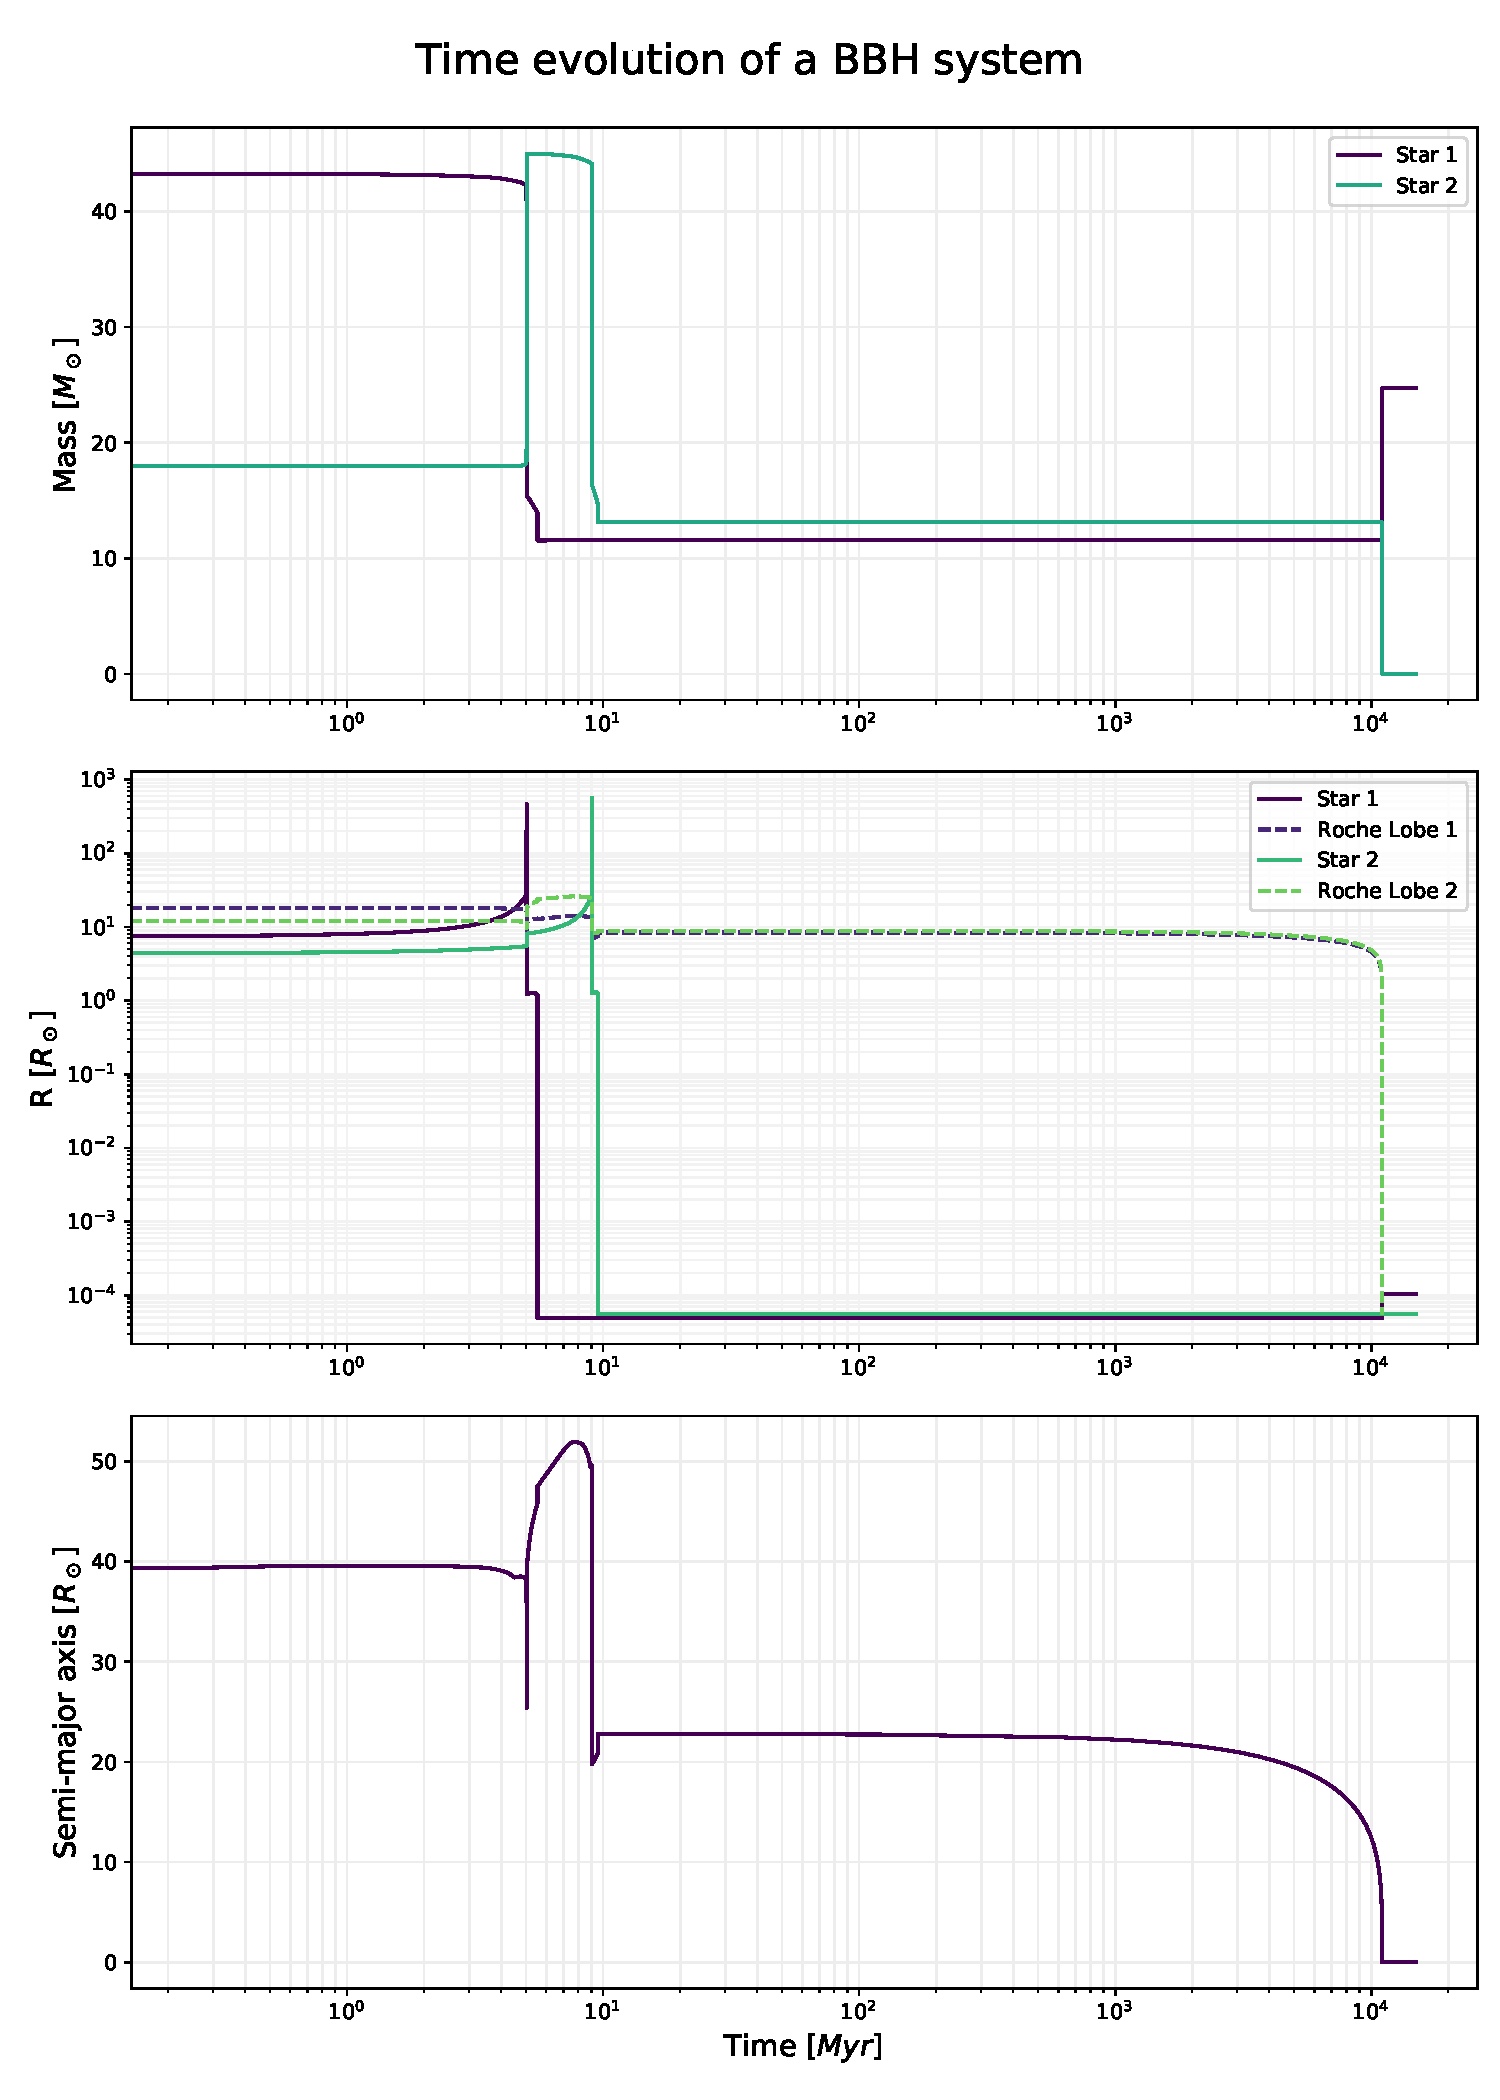
\includegraphics[width=0.9\textwidth]{images/method/time_evolution.pdf}
    \caption{Time evolution of a Binary Black Holes system. Top: mass of the two stars. Middle: radius and Roche Lobe radius of the two stars. Bottom: semi-major axis. }
    \label{fig:time_evolution}
    \end{minipage}
\end{figure}

\begin{figure*}[htp]
    \centering 
    %\begin{minipage}[c]{2.0\columnwidth}
    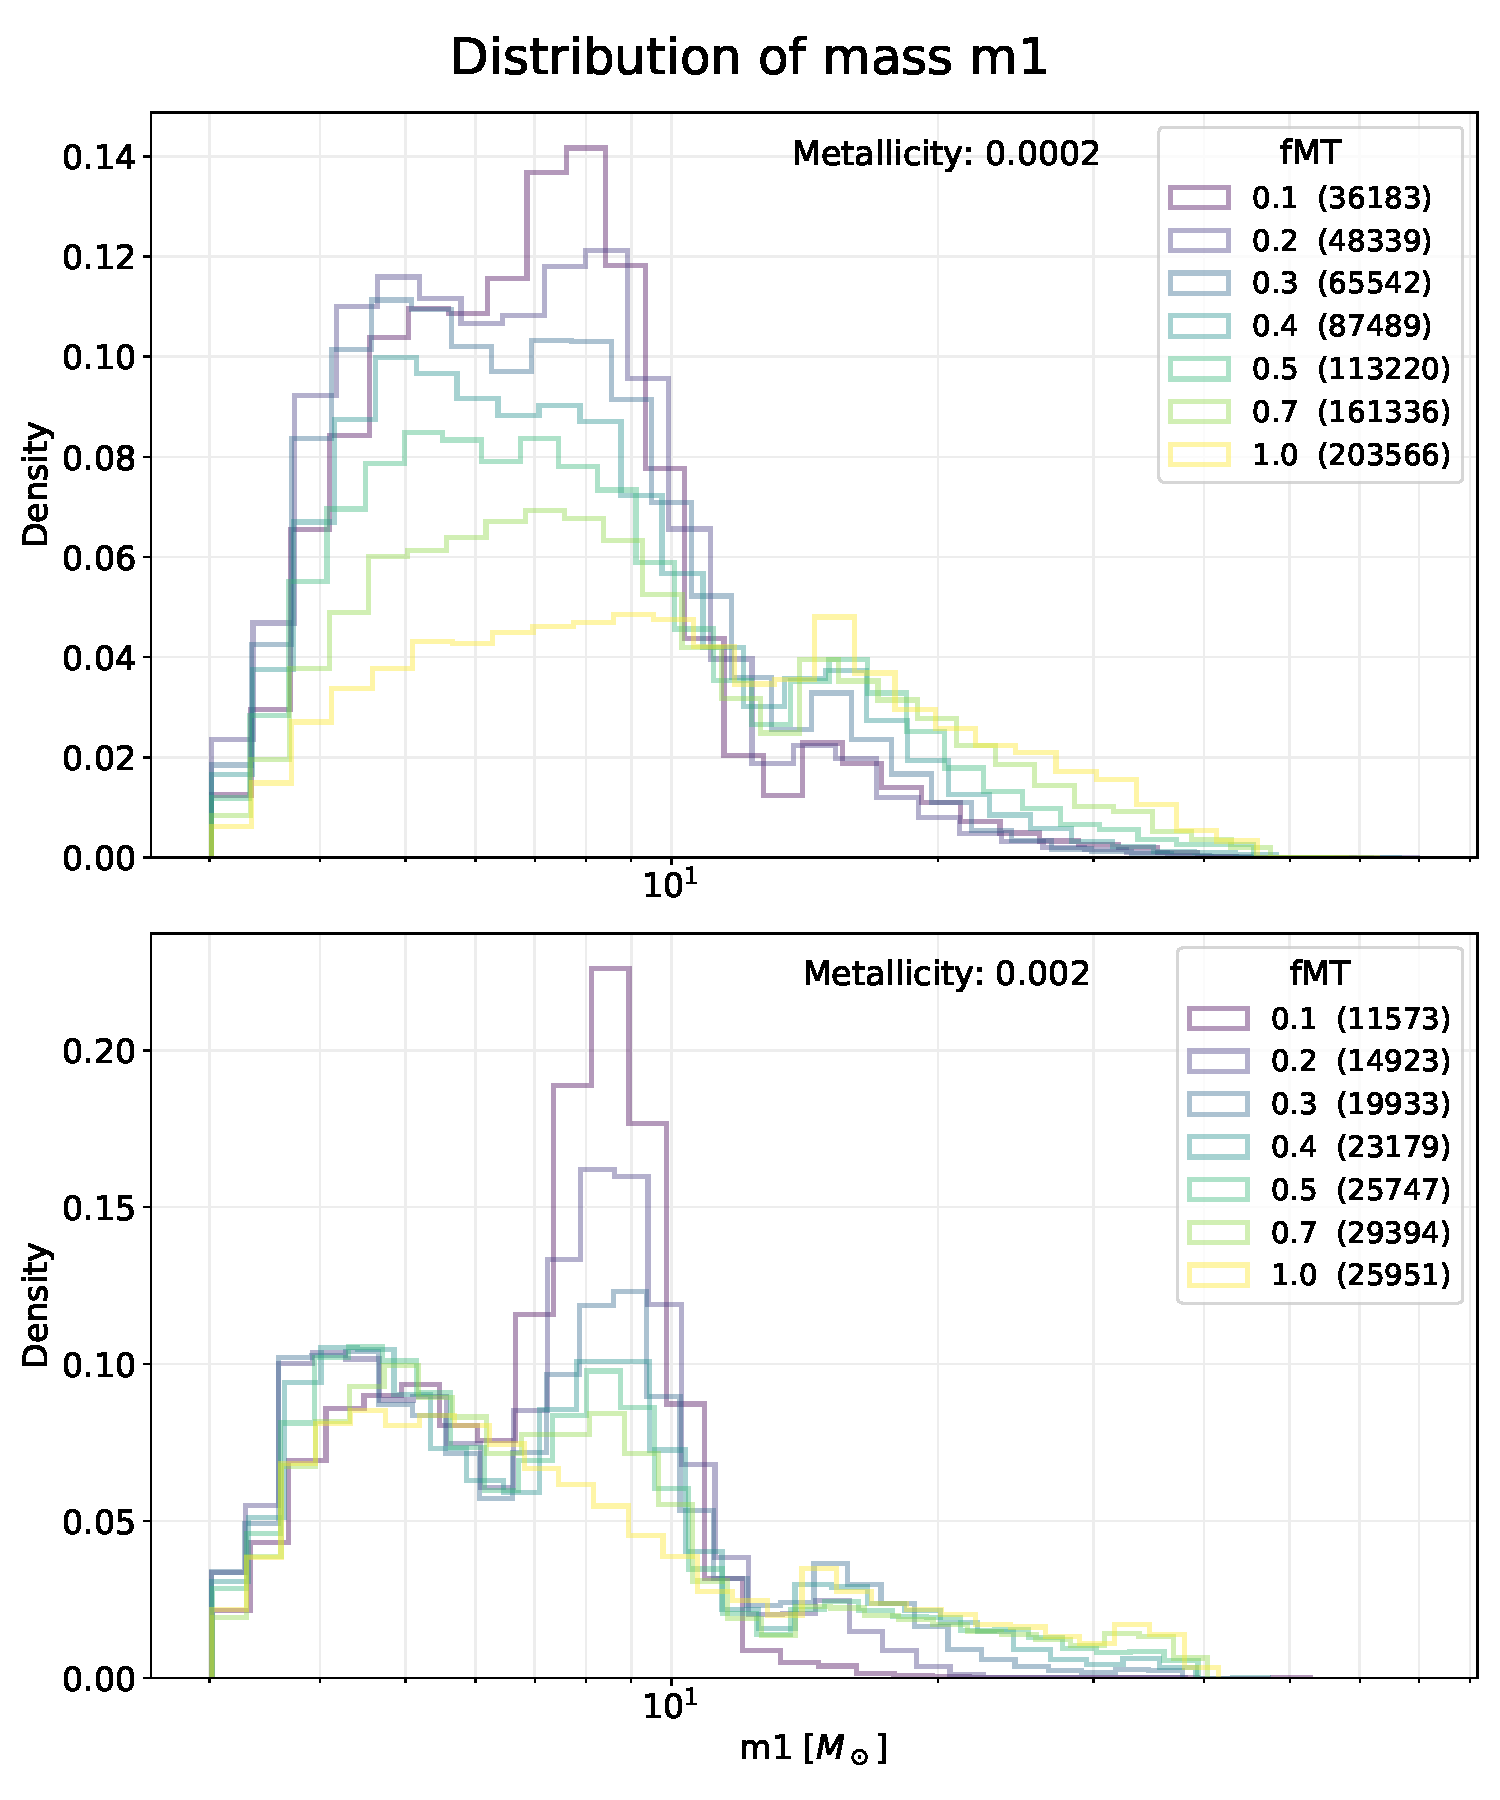
\includegraphics[width=0.49\textwidth]{images/assignment1/hist_mass_1.pdf}
    \hskip 1mm
   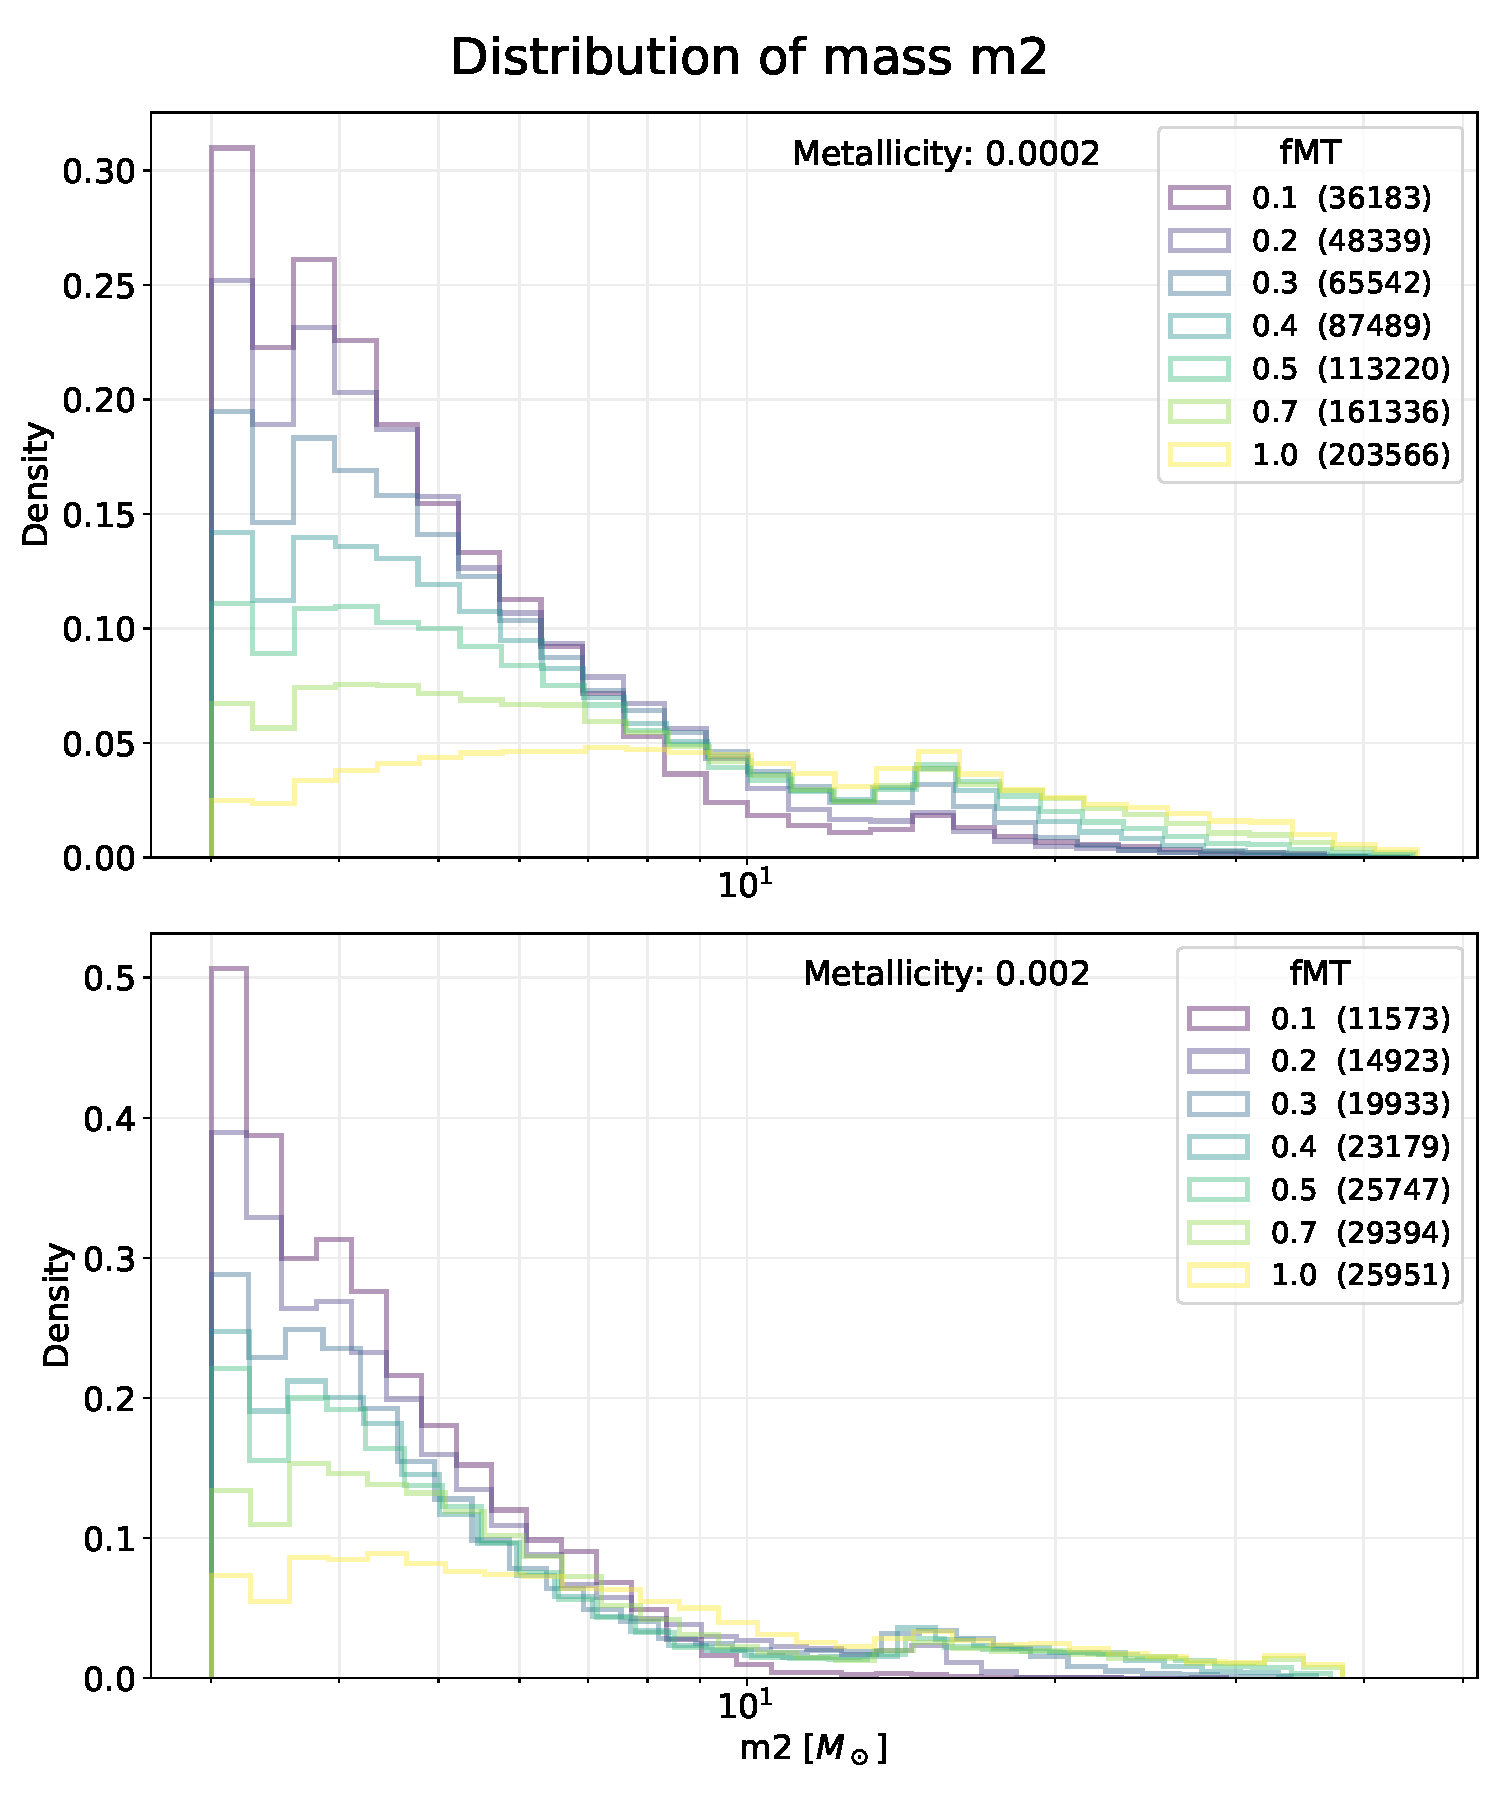
\includegraphics[width=0.49\textwidth]{images/assignment1/hist_mass_2.pdf}
    \\
    \vskip 0.7cm
    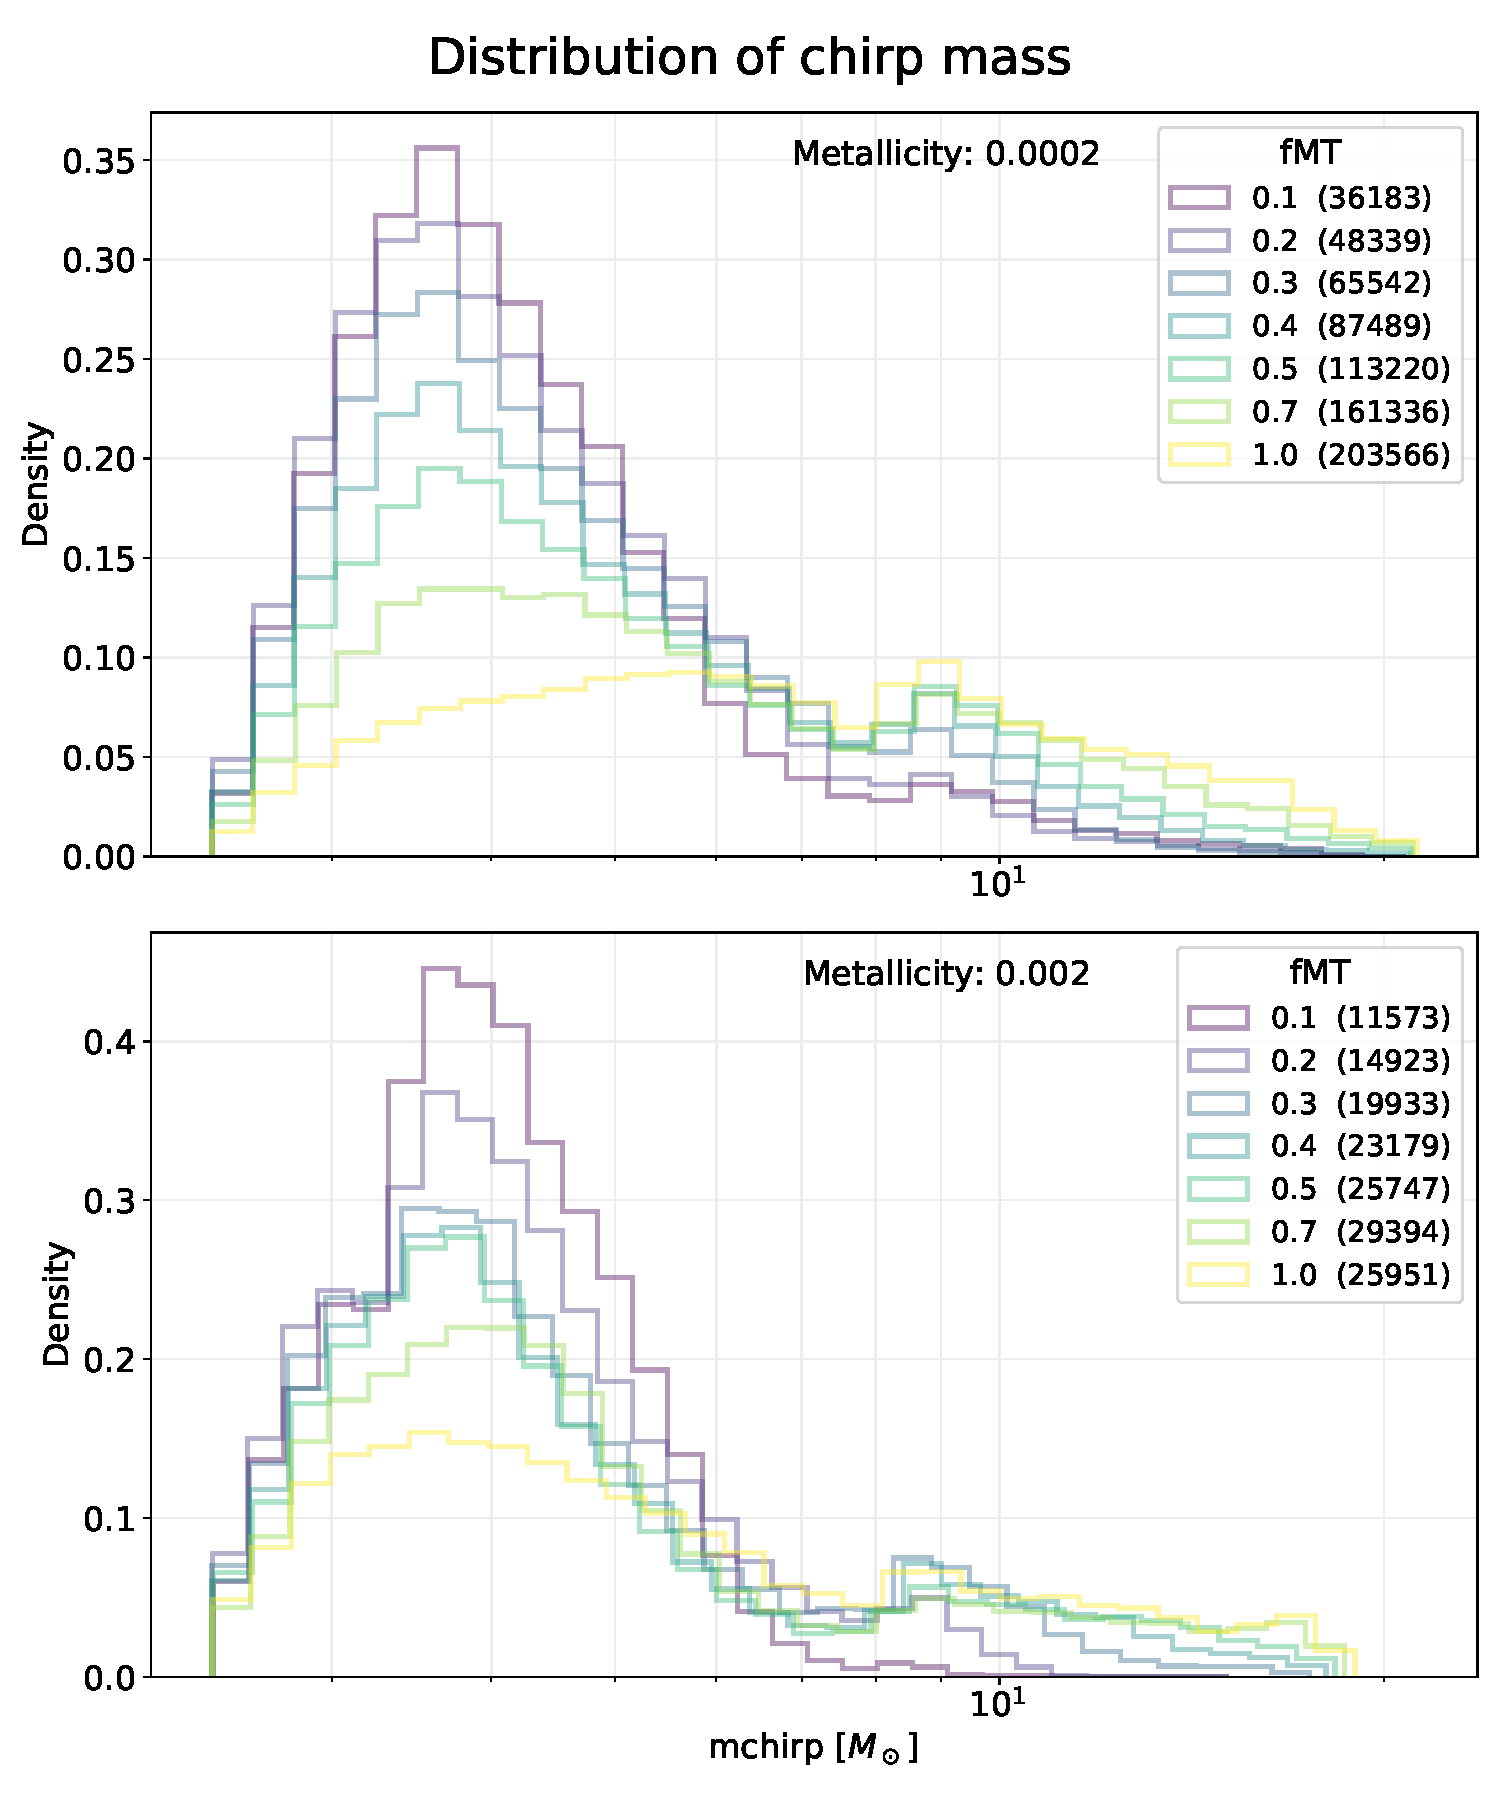
\includegraphics[width=0.49\textwidth]{images/assignment1/hist_mass_chirp.pdf}
   \hskip 1mm
   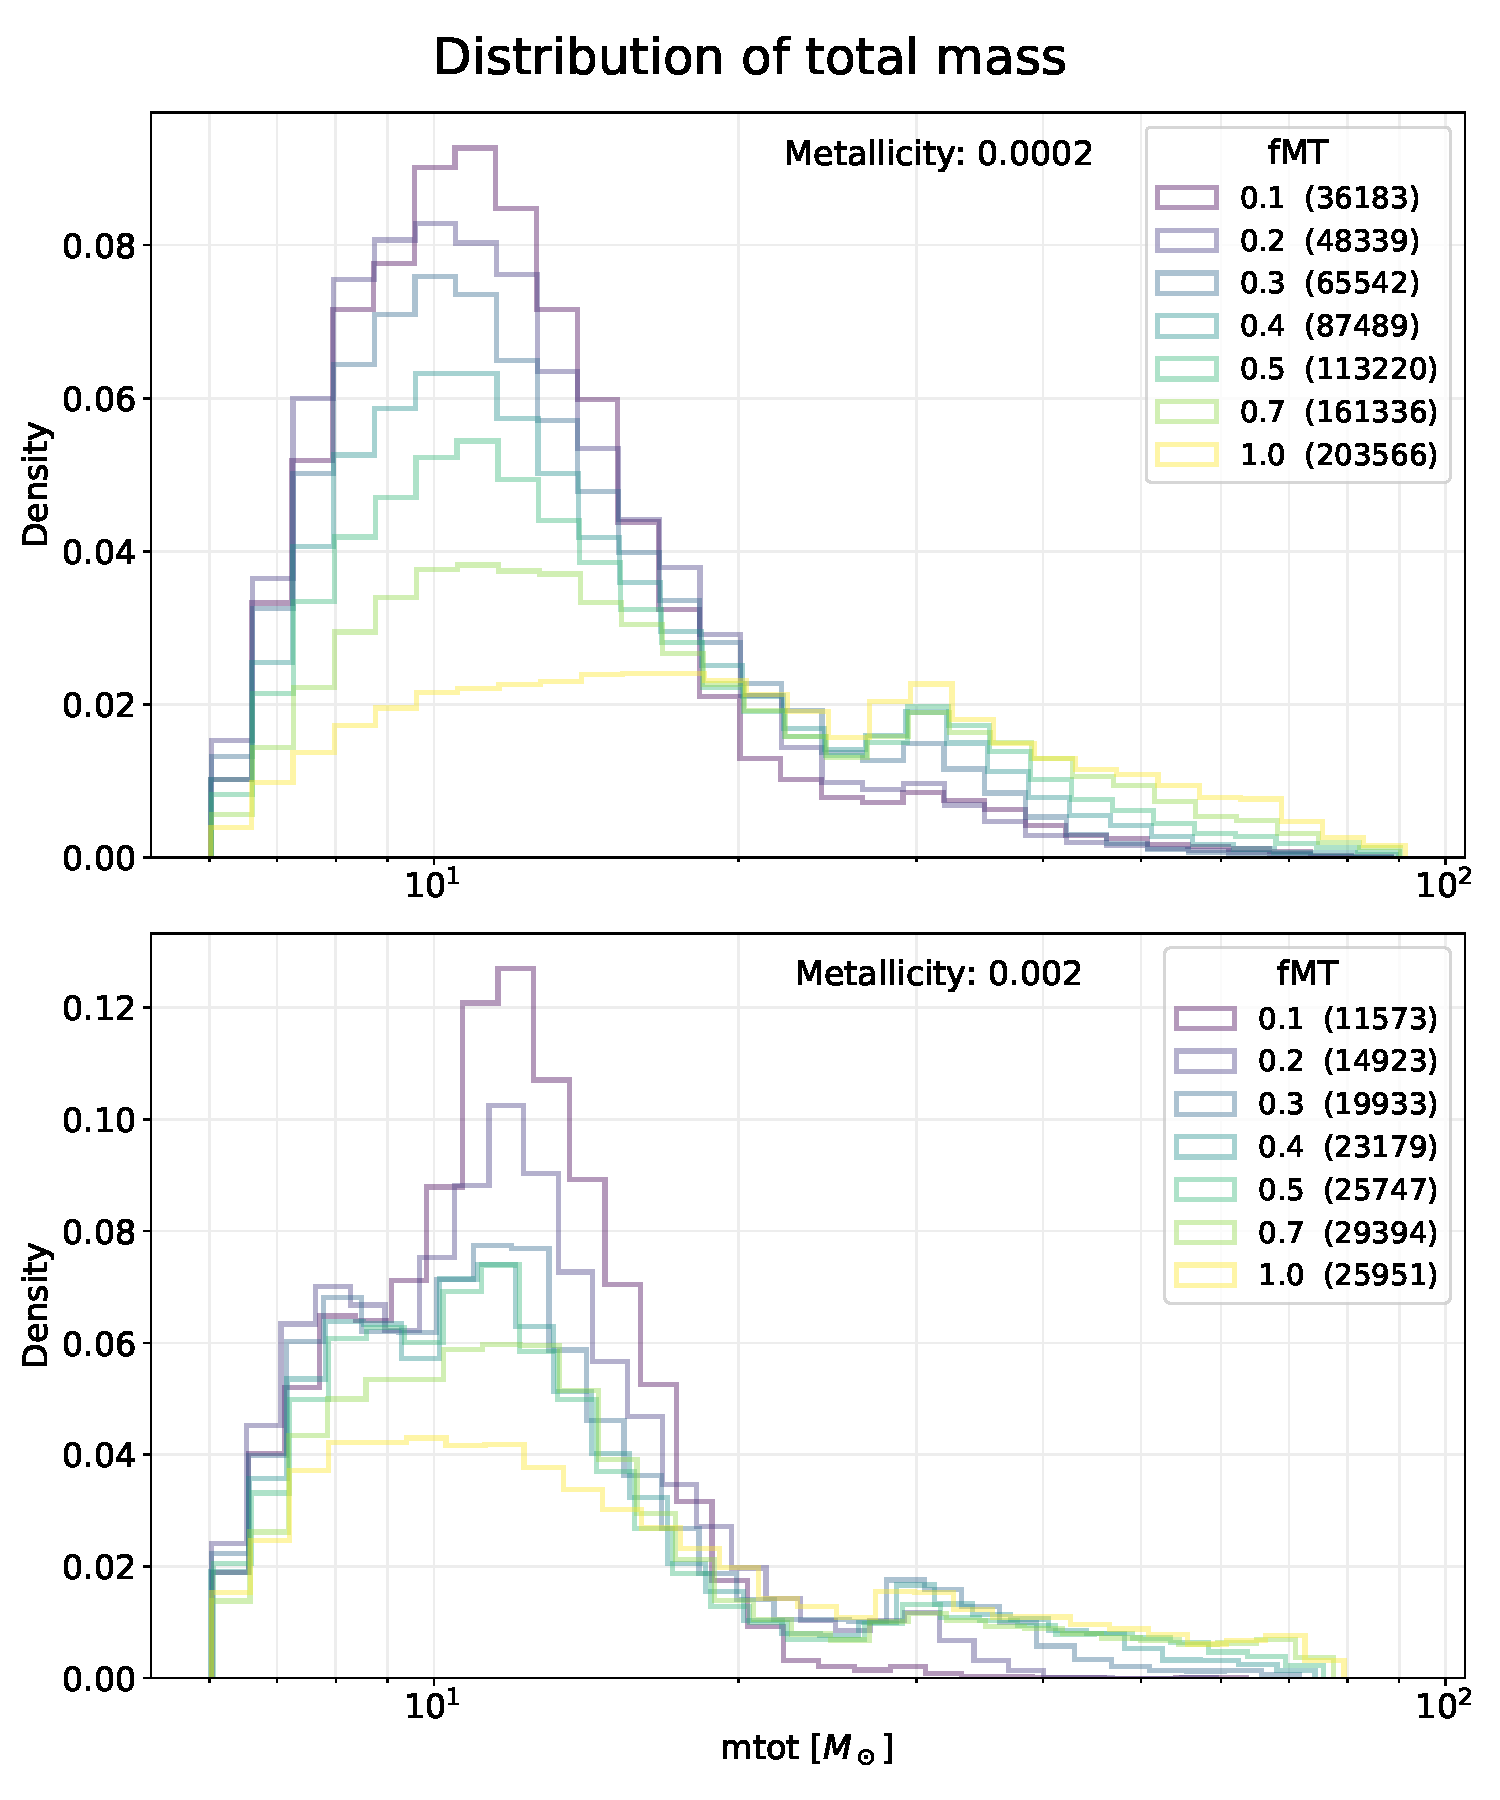
\includegraphics[width=0.49\textwidth]{images/assignment1/hist_mass_tot.pdf}
   \vskip 0.3cm
    \caption{Distribution of mass \(m_1\), \(m_2\), chirp mass and total mass as a function of fMT. In particular, for each set of distribution, on the top plots are illustrated the normalized histograms for metallicity of 0.0002, while on the bottom for metallicity of 0.002. In the legend, the color related to each fMT is reported  with the associated number of counts of the histograms.}
    \label{fig:ass1_masses}
    %\end{minipage}
\end{figure*}

\subsection{Data analysis}
We merge the data in the five different chunks for every metallicity and every fMT. 
For higher metallicities we expect to have few Binary Black Holes systems due to the fact that at higher metallicity stellar winds  lead to less massive stars. Therefore, we merge 0.012, 0.016 and 0.02 metallicities in order to increase the amount of data.

We plot the distribution of masses for different metallicities and fMT:
\begin{itemize}
    \item \(m_1\): mass of the primary compact object before merging;
    \item \(m_2\): mass of the secondary compact object before merging;
    \item \(m_{\text{chirp}} \): main mass parameter experimentally derived from the frequency during in-spiral
        \begin{equation*}
            m_{\text{chirp}} = \frac{(m_1 m_2)^{3/5}}{(m_1+m_2)^{1/5}};
        \end{equation*}
   \item \( m_{\text{tot}}\): total mass, it is in particular given by the information at merger \( m_{\text{tot}}  = (m_1+m_2) \);
   \item \(q\): mass ratio \(q  = m_2/m_1 \).
\end{itemize}
Then, we plot the distribution of \(t_{\text{merg}}\),  which is the time to merge by gravitational waves emission. Since we observe a linear behavior in log-log scale, we suppose that the distribution of \(t_{\text{merg}}\) is a power-law and we fit it. 
Moreover, we plot the fraction of systems in which the primary star evolves in the secondary compact object and vice versa as a function of fMT merging all metallicities.

After that, we distinguish between systems that go through Common Envelope (CE) and the ones that do not (nCE). In this case we merge all metallicities lower or equal than 0.002.
We plot the fraction of CE systems as a function of fMT.
We analyze the differences between their distributions of initial masses (i.e. the mass at the beginning of the main sequence), final masses (i.e. the mass of the compact object), mass ratios and delay times. 
Moreover, we plot the scatter plots of the two masses forming the binaries at the beginning and at the end of the evolution. 
Eventually, we plot the distributions of semi-major axis for different metallicities and fMT.



%%%%%%%%%%%%%%%%%%%%%%%%%%%%%%%%%%%%%%%%%%%%%%%%%%%%%%%%%%%%%%%%%%%%%
\section{Results}
\label{sec:results}

In Fig. \ref{fig:ass1_masses} we plot the distribution of \(m_1\), \(m_2\), \(m_\text{chirp}\) and \(m_\text{tot}\). We show histogram for two relevant metallicities, \(0.0002\) and \(0.002\); in particular we observe that for higher metallicities the number of counts decrease to the point where it is not enough to have a meaningful distribution. 
First of all we consider primary and secondary mass distributions, we observe that \(m_1\) is peaked around \SI{10}{\(M_{\odot}\)} while the peak of \(m_2\) distribution is found around few \(M_{\odot}\). In both cases, for higher values of fMT, a second smaller peak emerges from the right tail of the distribution. 
Since Common Envelope ejection cause a significant loss of mass, the latter is populated by nCE systems which, in particular if the mass transfer is very efficient, gain more mass and produces heavier Black Holes. %, as shown in Fig. \ref{fig:ass2_masses}. 

Moreover, increasing fMT the relative frequency of low mass Black Holes decreases lowering the height of the peak. In fact, with higher efficiency, the binary system loses a smaller fraction of its initial mass producing generally more massive compact objects. 
Eventually, the distributions of \(m_\text{chirp}\) and \(m_\text{tot}\) substantially show the same trend of the primary mass distribution due to the fact that the heavier star of the system dominates the trend of reduced and total mass.

%\onecolumngrid

%\twocolumngrid

%\clearpage
\begin{figure}[!t]
    \begin{minipage}[l]{1.0\columnwidth}
    \centering
    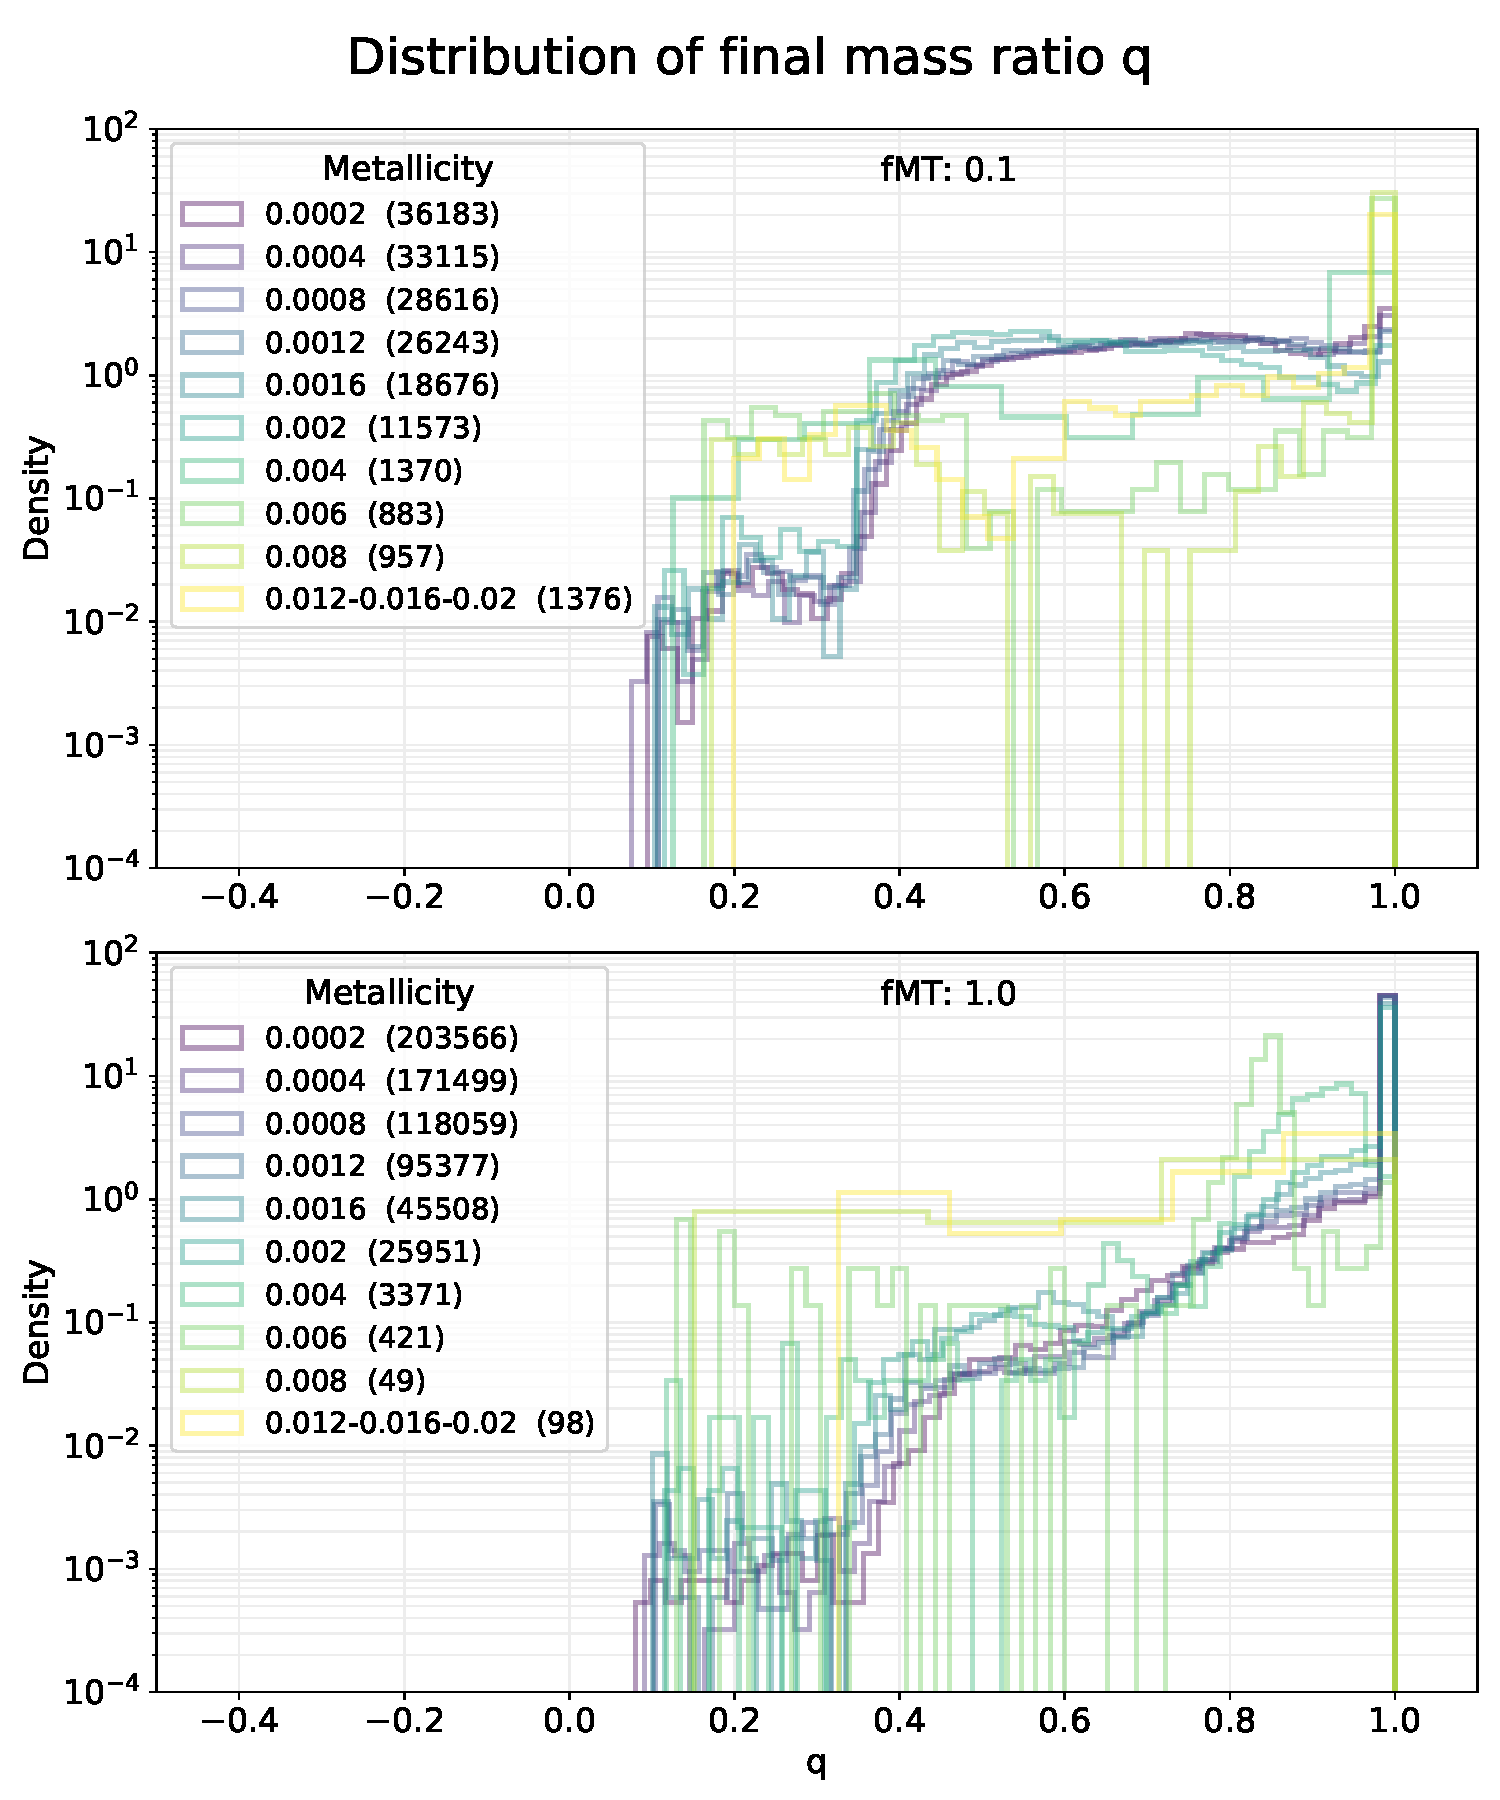
\includegraphics[width=0.9\textwidth]{images/assignment1/mass_ratio_2.pdf}
    \caption{Distribution of mass ratio \(q=m_2/m_1\) for different values of the metallicity. On the top, we illustrate the distribution of mass ratio for systems with fMT\(=1\), while on the bottom for systems with fMT\(=0.1\). 
    }
    \label{fig:ass1_histq}
    \end{minipage}
    %\vspace{-1cm}
\end{figure}

In Fig. \ref{fig:ass1_histq} we plot the distribution of the mass ratio \(q\) for fMT\(=0.1\) and fMT\(=1\) varying the metallicity. We observe that for low mass transfer efficiency the distributions for higher metallicities are more peaked around one; while for efficient mass transfer the distributions for lower metallicities are peaked around one. In fact, for fMT\(\sim 1\) the secondary accretes the whole mass lost by the primary and for high metallicity, due to significant mass loss by stellar wind, lower mass Black Holes are produced with mass ratio further from one. On the contrary, for fMT\(\sim 0.1\) the secondary can not accrete the whole mass lost by the primary and for low metallicity we observe more massive Black Holes with mass ratio further from one.

%We observe that for lower metallicities the left tail of the distribution vanish around 0.4, while increasing the metallicity systems show more extreme mass ratios. This trend is due to the fact that at higher metallicity mass loss is more relevant for both stars and the ratio gets further and further from one. 
%Moreover increasing fMT, the distribution gets more and more peaked at \(q=1\); in fact, if the mass transfer is more efficient, stars tends to balance their masses. 

%\begin{figure}[!t]
%    \begin{minipage}[l]{1.0\columnwidth}
%    \centering
%    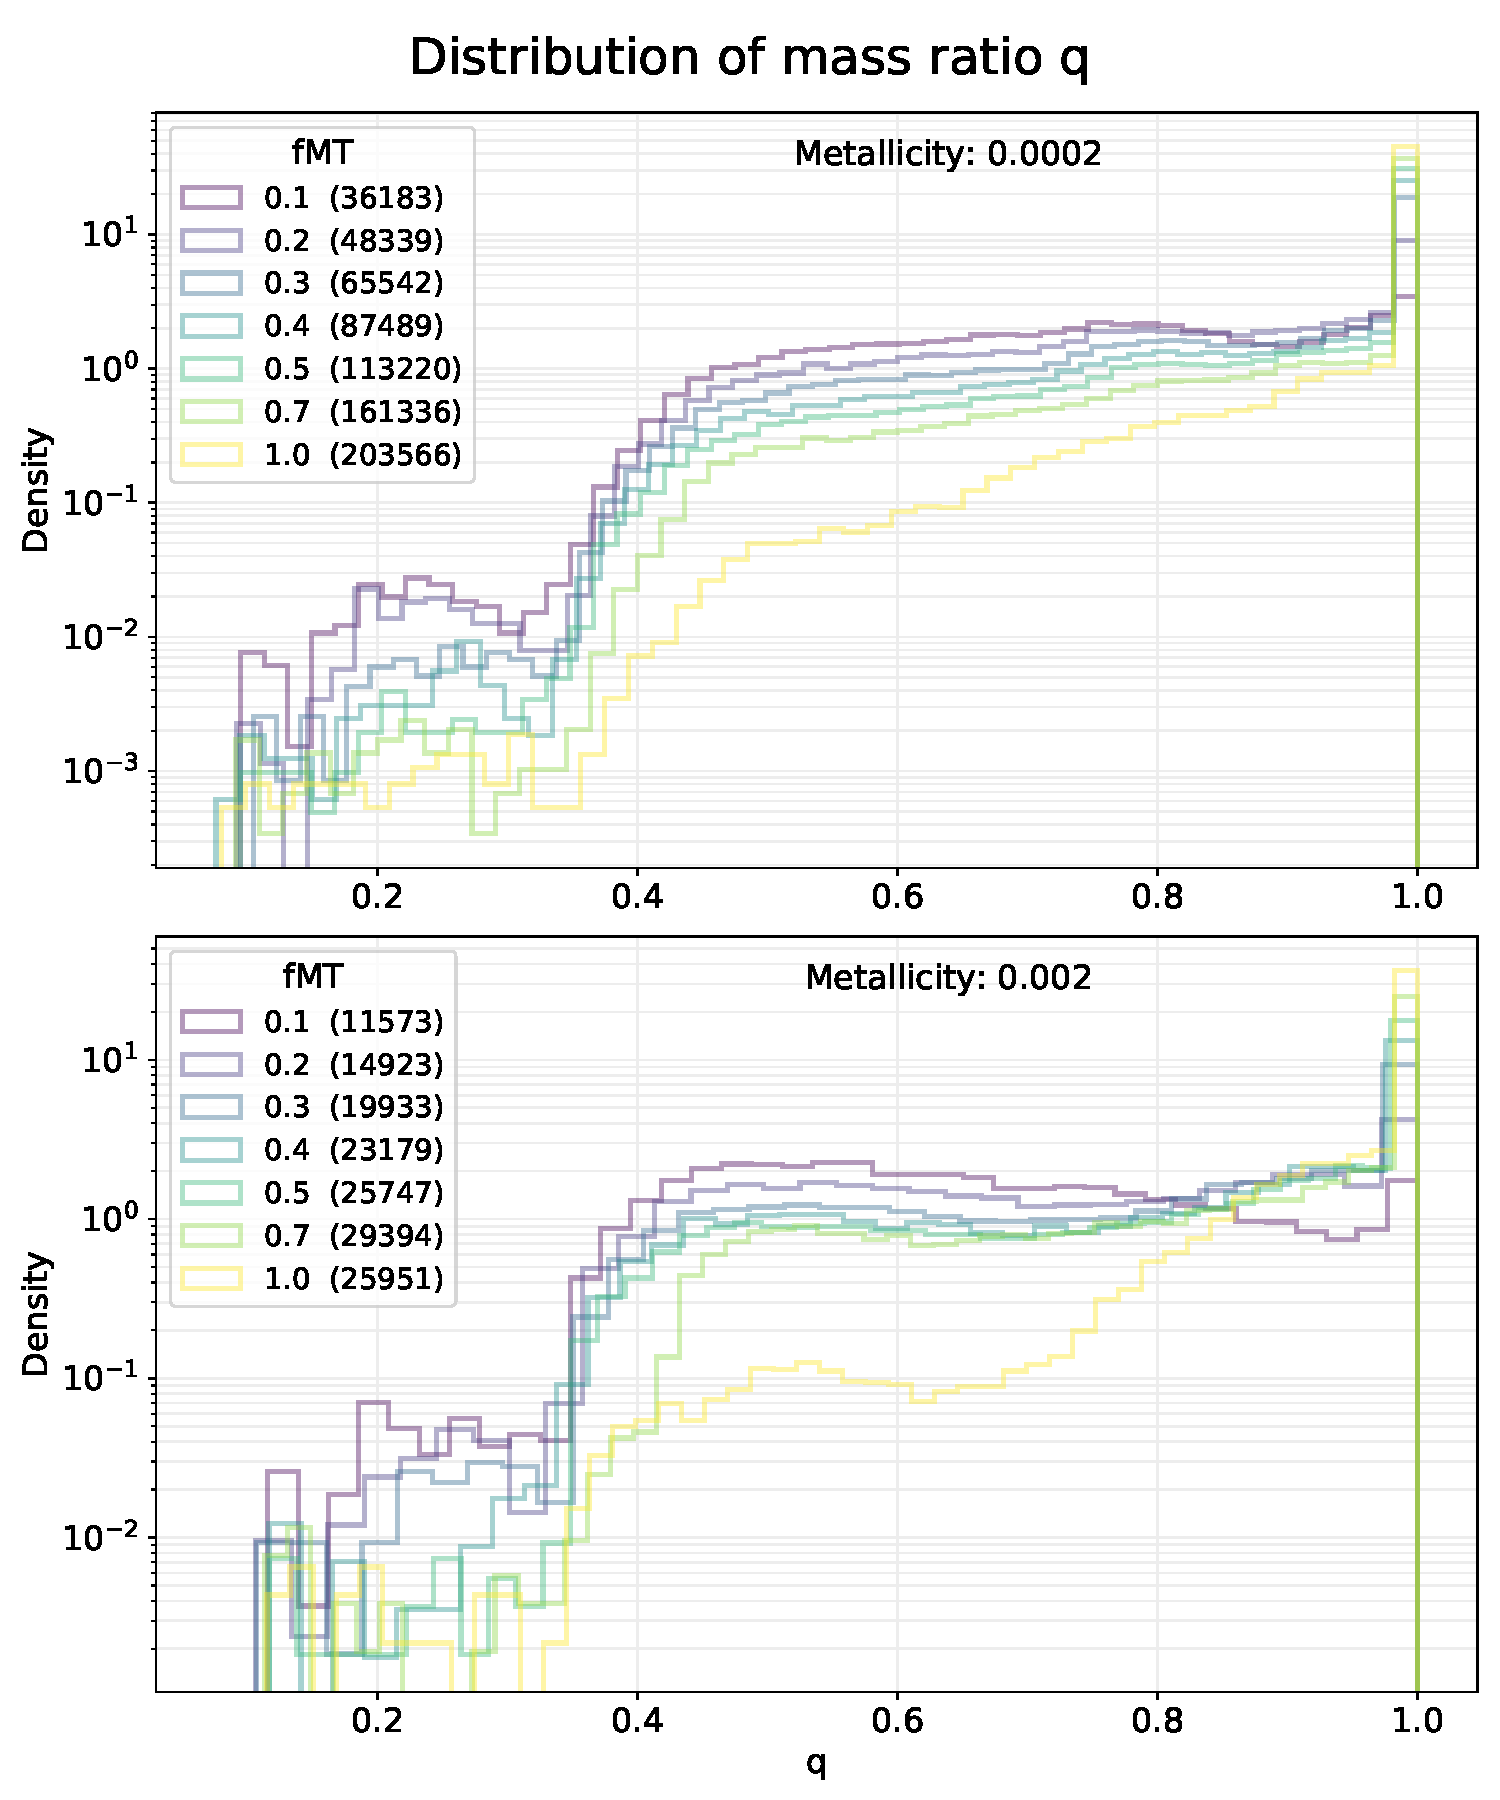
\includegraphics[width=0.9\textwidth]{images/assignment1/hist_q.pdf}
%    \caption{Distribution of mass ratio \(q=m_2/m_1\), where \(m_1\) is the most massive Black Hole, for different fMT. On the top, the plot for metallicity equal to 0.0002 is illustrated, while on the bottom for 0.002. In the legend, the color related to each  fMT is reported  with the associated number of counts of the histograms.}
%    \label{fig:ass1_histq}
%    \end{minipage}
%    \vspace{-0.1cm}
%\end{figure}

\begin{figure}[hbp]
    \begin{minipage}[l]{1.0\columnwidth}
    \centering
    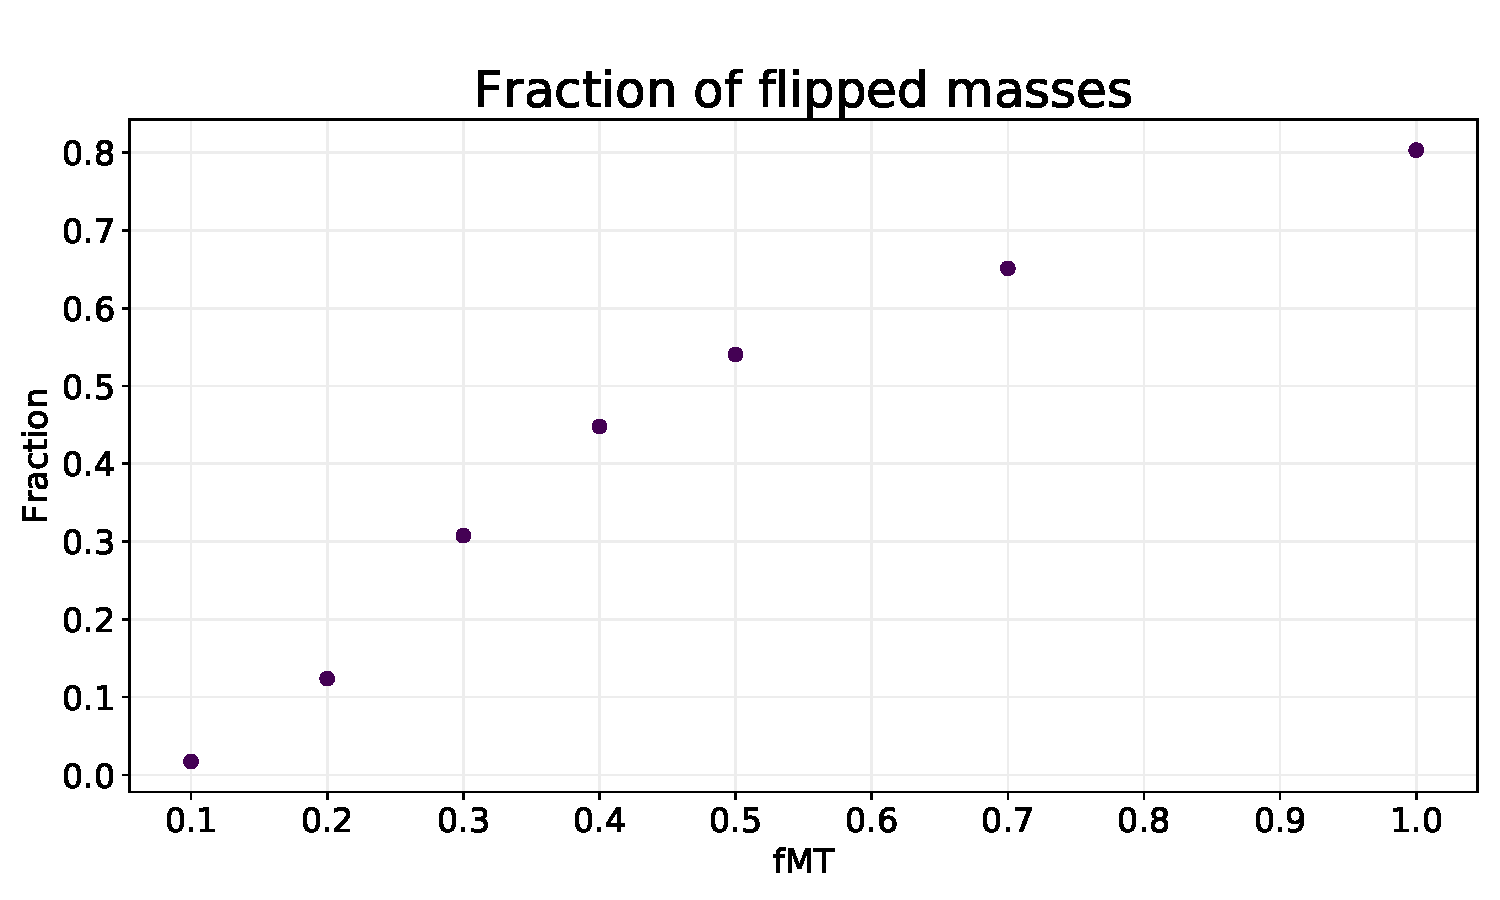
\includegraphics[width=0.9\textwidth]{images/assignment1/fraction_fMT.pdf}
    \caption{Fraction of Binary Black Holes systems with flipped masses as a function of fMT.}
    \label{fig:ass1_fraq_fmt}
    \end{minipage}
\end{figure}

\begin{figure}[htp]
    \begin{minipage}[l]{1.0\columnwidth}
    \centering
    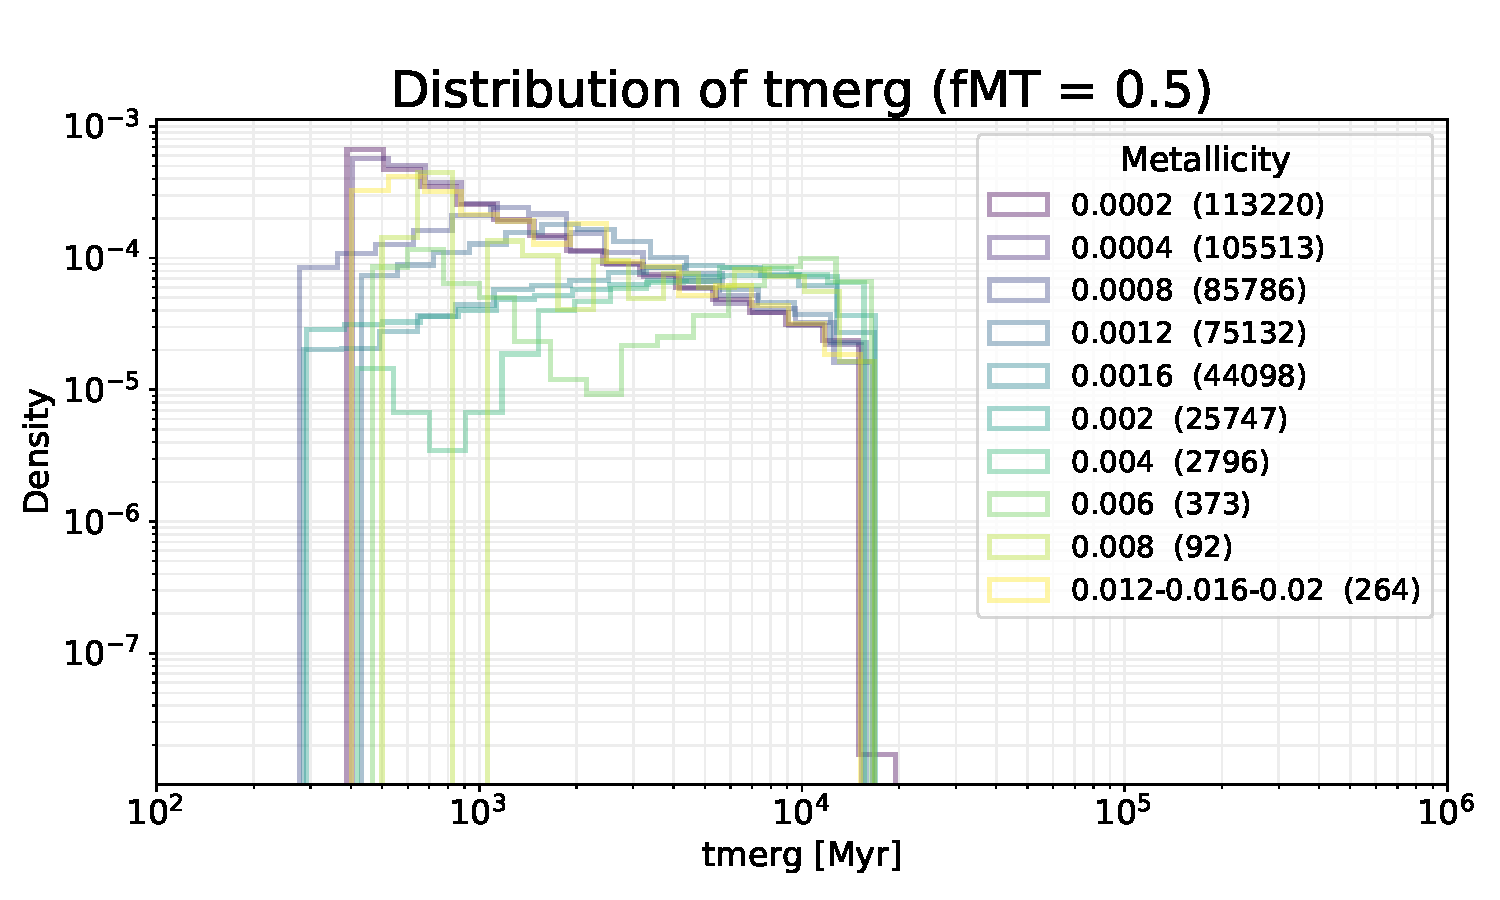
\includegraphics[width=0.9\textwidth]{images/assignment1/hist_time_tmerg.pdf} \\
     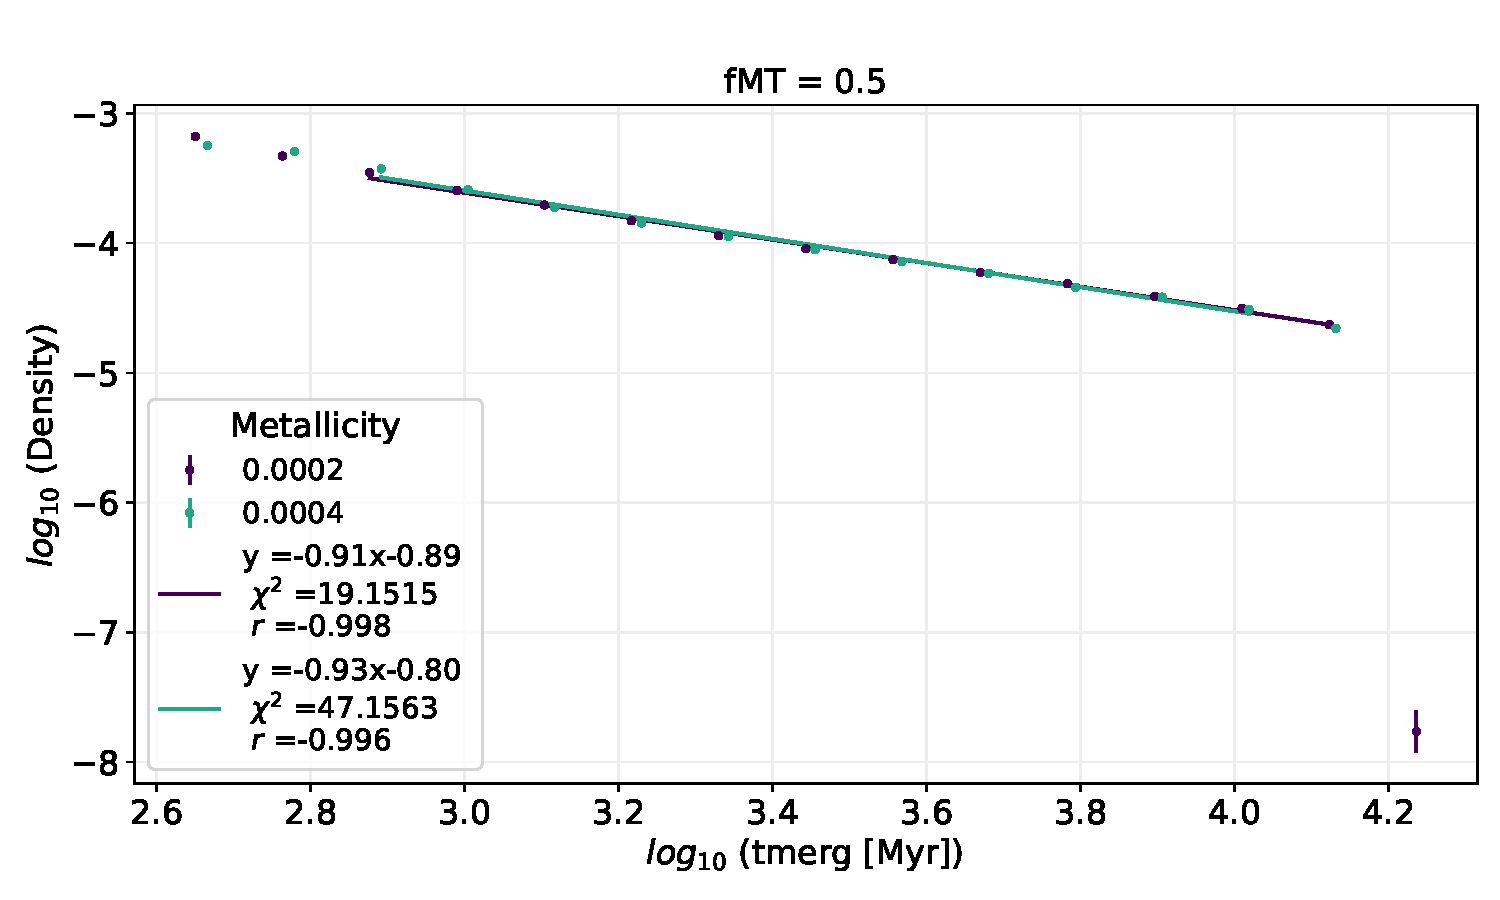
\includegraphics[width=0.9\textwidth]{images/assignment1/fit_hist_time_tmerg.pdf}
    \end{minipage}
    \caption{On the top, the distribution of merging times for different metallicities is illustrated for  fMT equal to 0.5. In the legend, the color related to each metallicity is reported  with the associated number of counts of the histograms. On the bottom, the linear fit of the distributions are illustrated for metallicity of 0.0002 and 0.0004.}
    \label{fig:ass1_tmerg}
\end{figure}

The fraction of flipped masses increases for higher fMT as shown in Fig. \ref{fig:ass1_fraq_fmt}; in fact, for more efficient mass transfer generally we have a greater exchange of mass.

Eventually, we observe no dependence on different fMT values in \(t_\text{merg}\) distribution. In Fig. \ref{fig:ass1_tmerg} we show the \(t_\text{merg}\) distribution for \( \text{fMT} = 0.5\) and different Z. We observe a power law distribution for lower metalicities, while the peak of the distribution moves toward higher delay times for higher ones. Indeed, for higher metallicities, we generally have less massive stars which have a slower evolution.

\begin{figure}[hp]
    \begin{minipage}[l]{1.0\columnwidth}
    \centering
    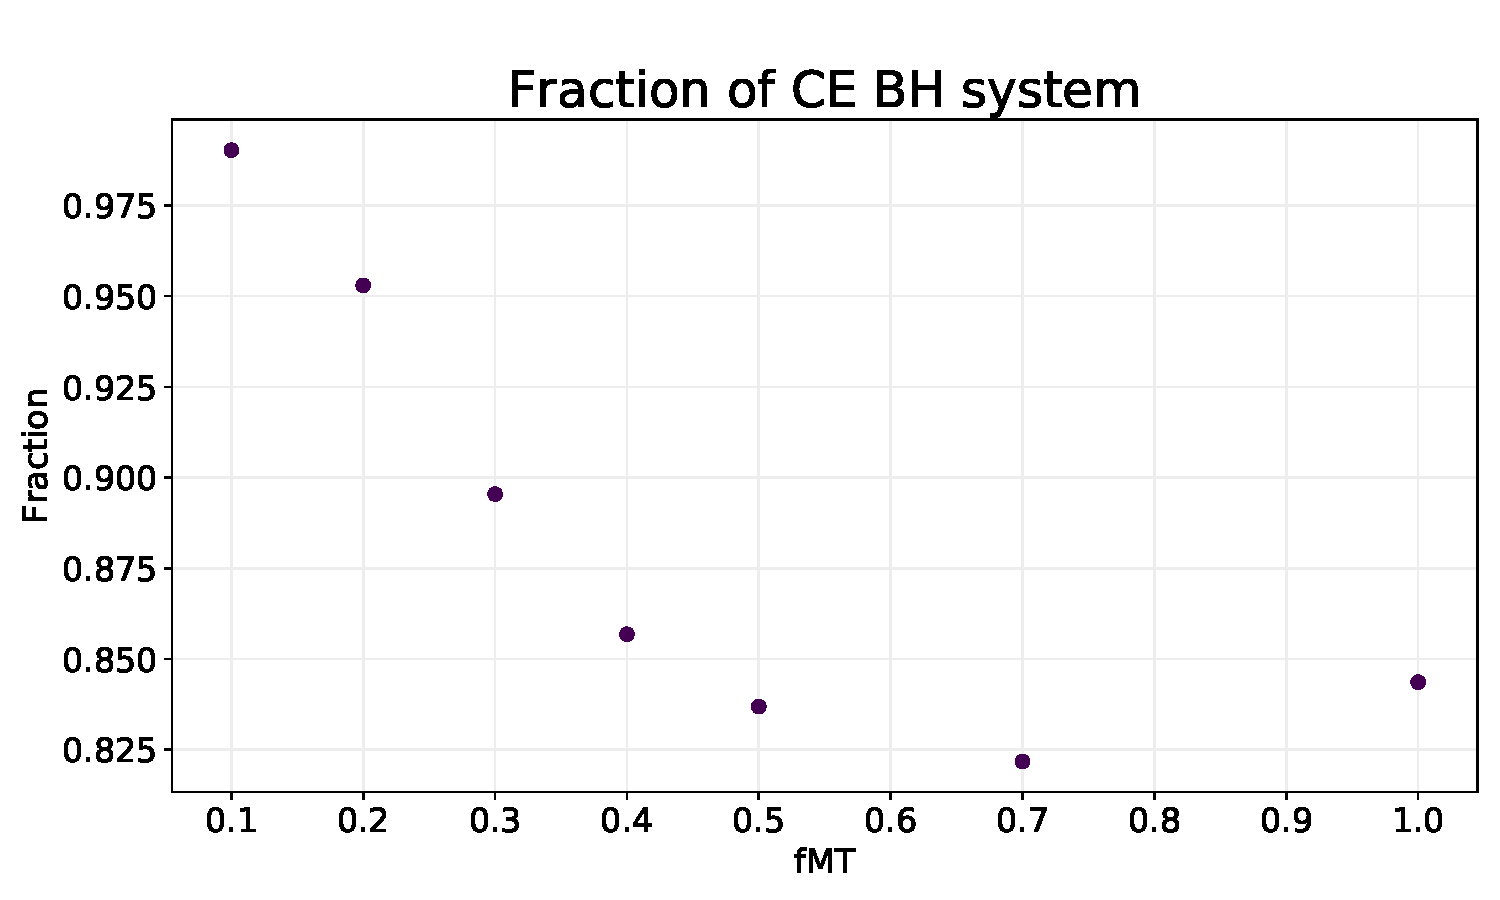
\includegraphics[width=0.9\textwidth]{images/assignment2/frac_CE.pdf}
    \caption{Fraction of Binary Black Holes systems which enter in Common Envelope as a function of fMT.}
    \label{fig:ass2_frac_CE}
    \end{minipage}
\end{figure}

\begin{figure*}[htp]
    \centering 
    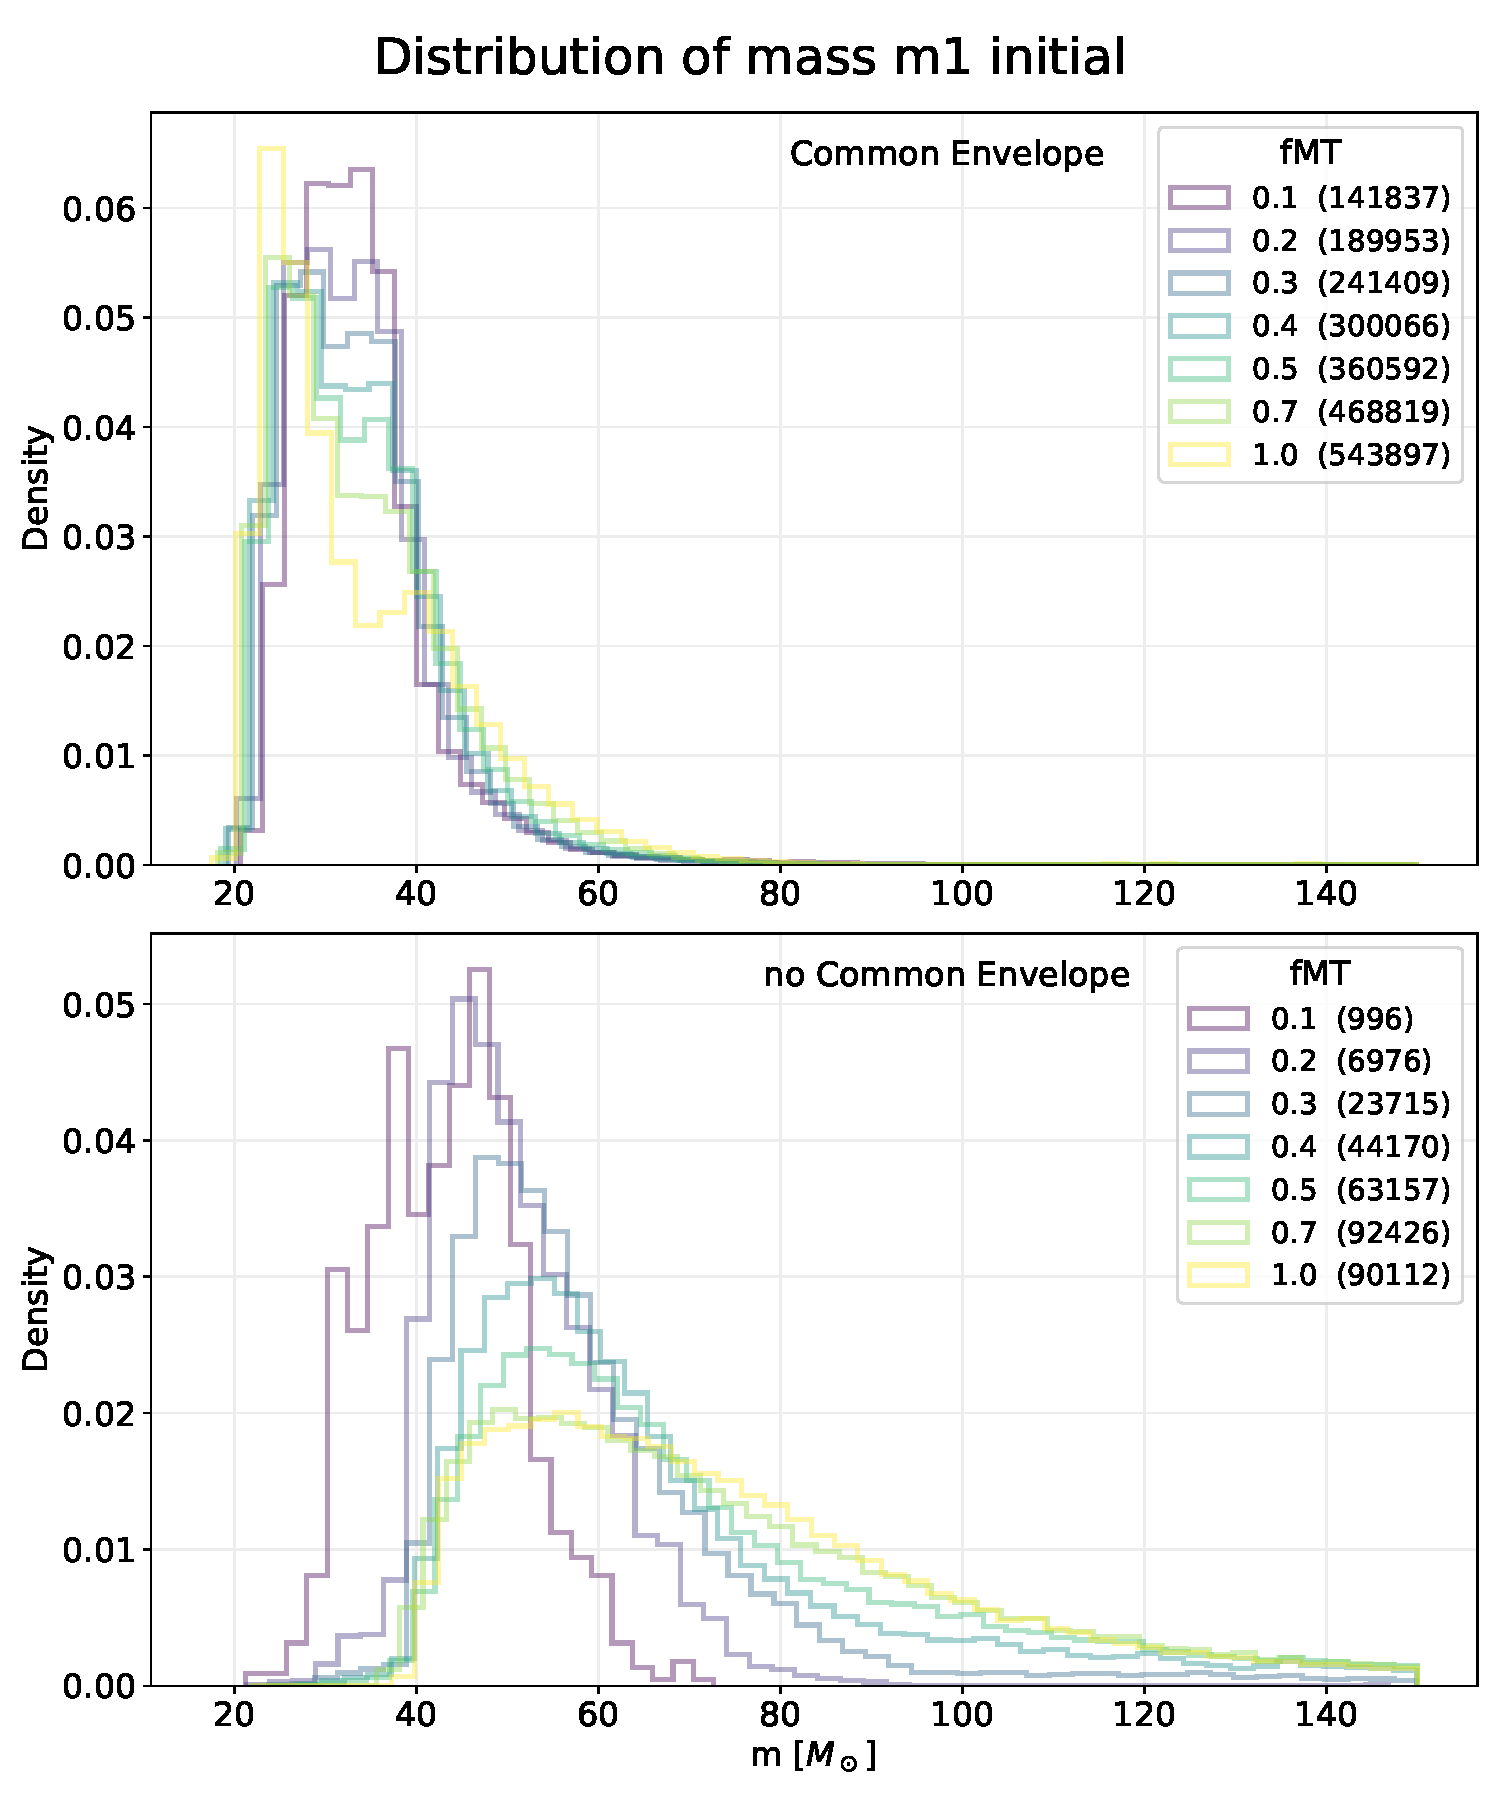
\includegraphics[width=0.49\textwidth]{images/assignment2_1/hist_m1_init_fMT.pdf}
    \hskip 1mm
   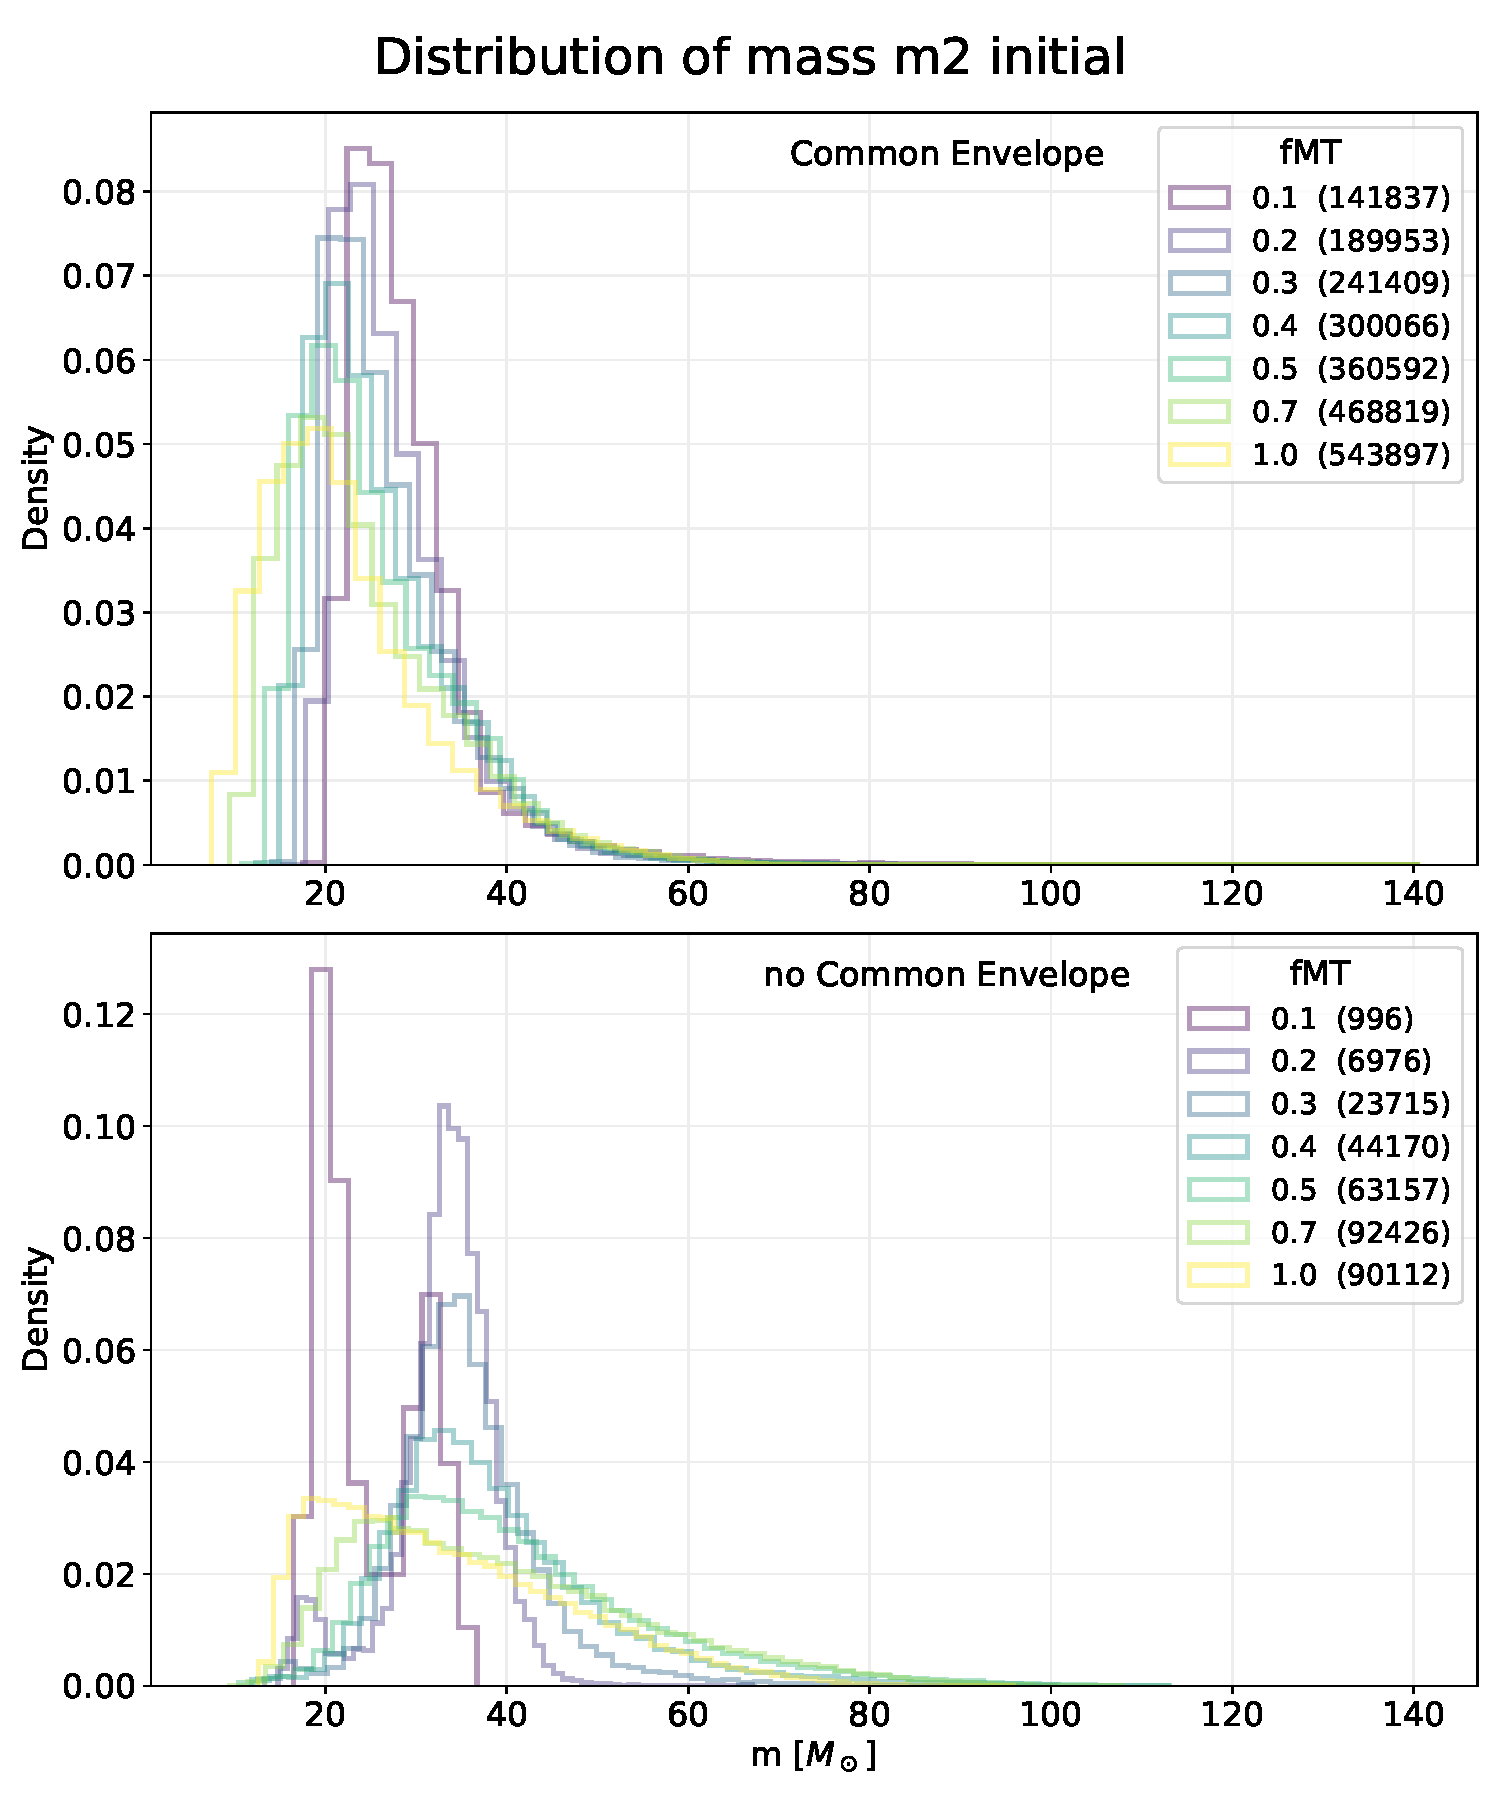
\includegraphics[width=0.49\textwidth]{images/assignment2_1/hist_m2_init_fMT.pdf}
    \\
    \vskip 0.7cm
    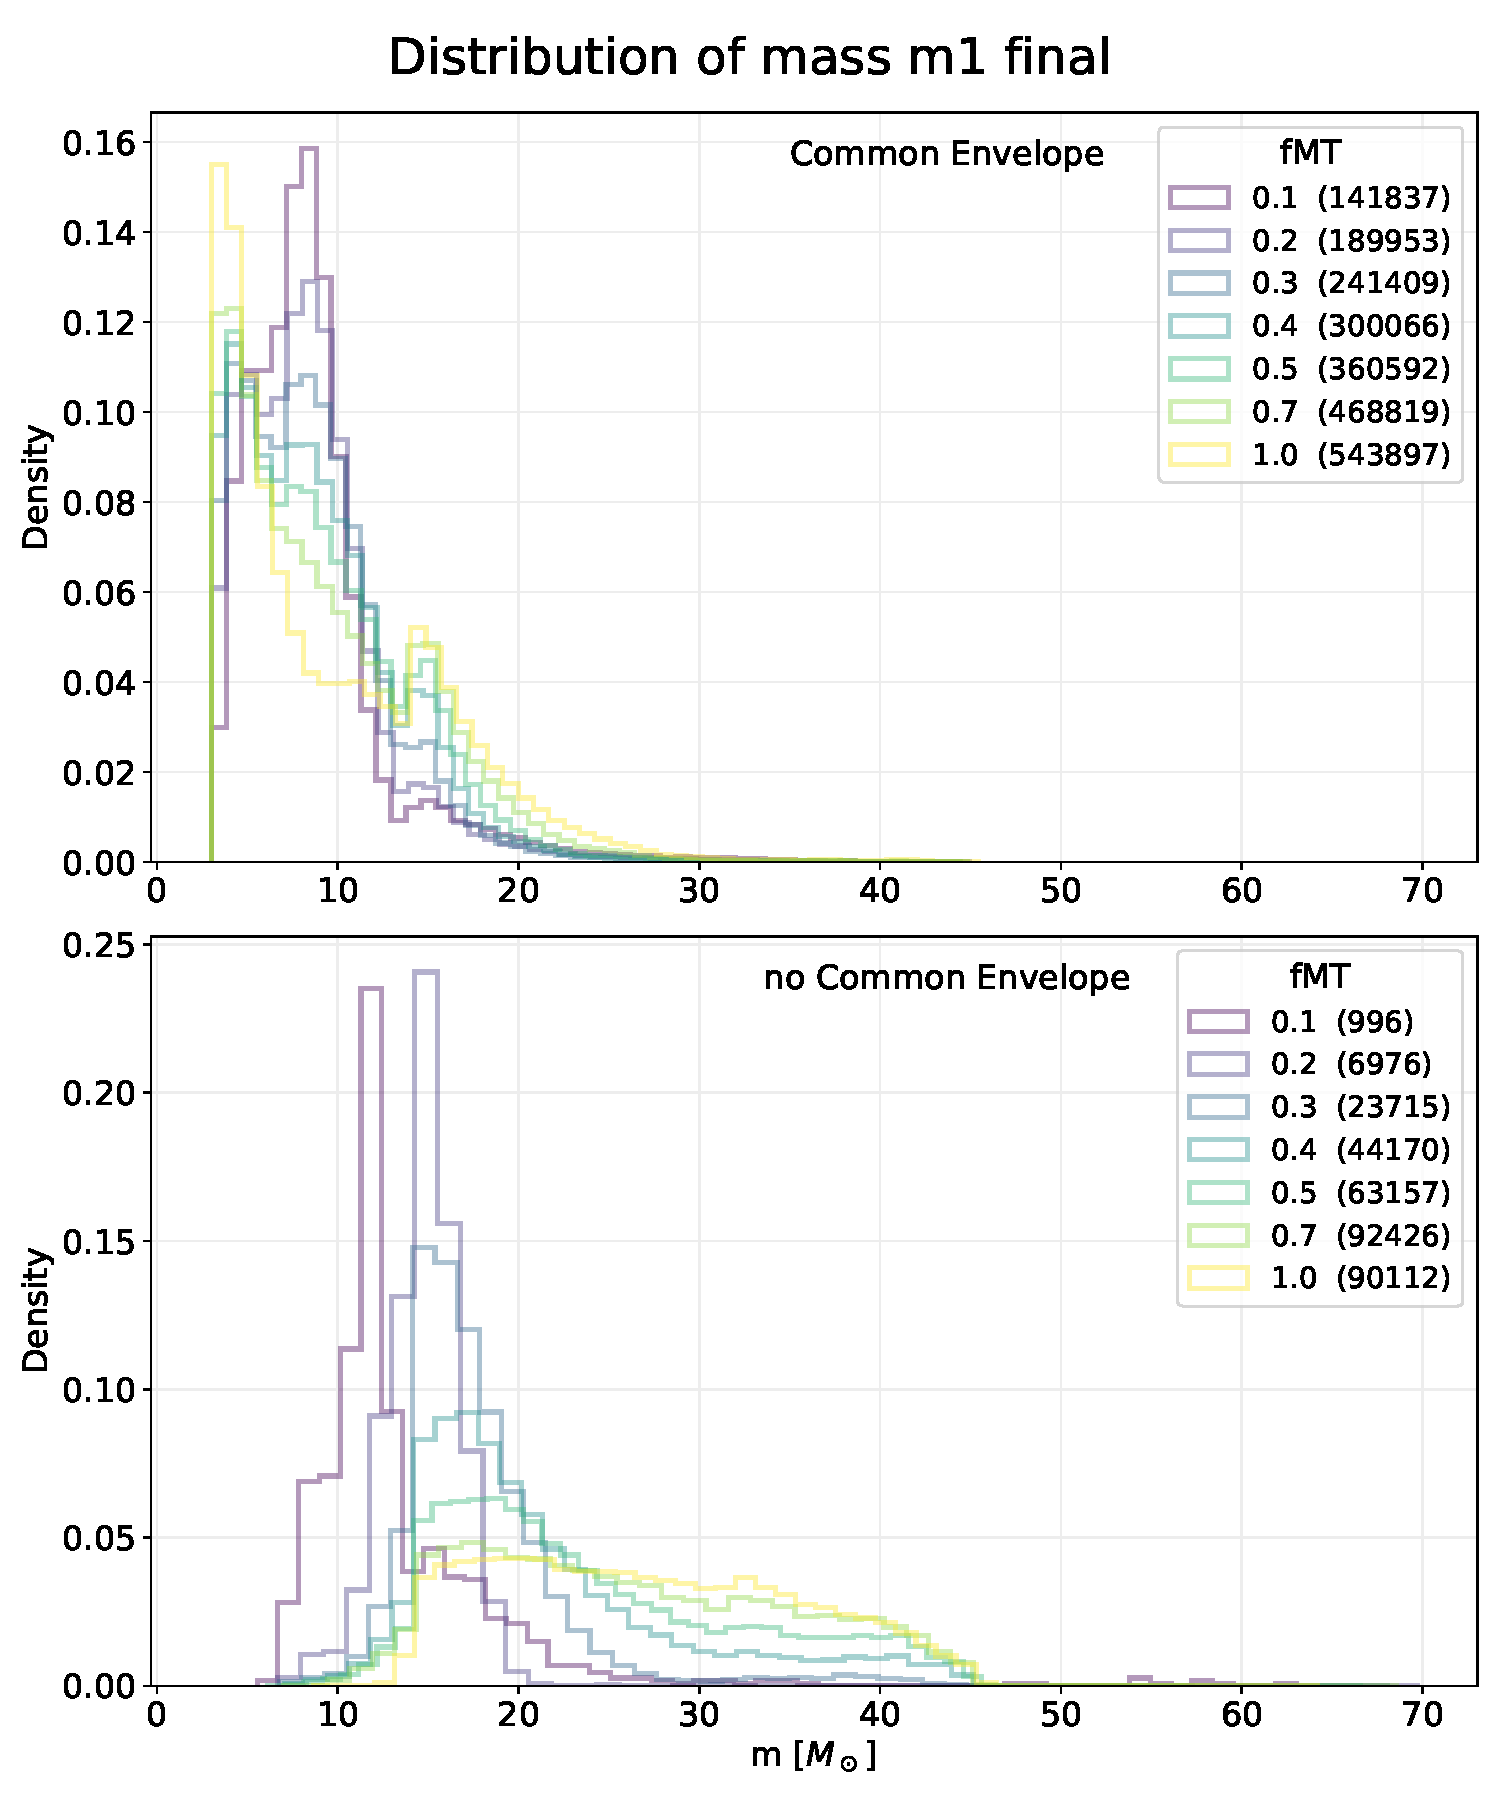
\includegraphics[width=0.49\textwidth]{images/assignment2_1/hist_m1_fin_fMT.pdf}
   \hskip 1mm
   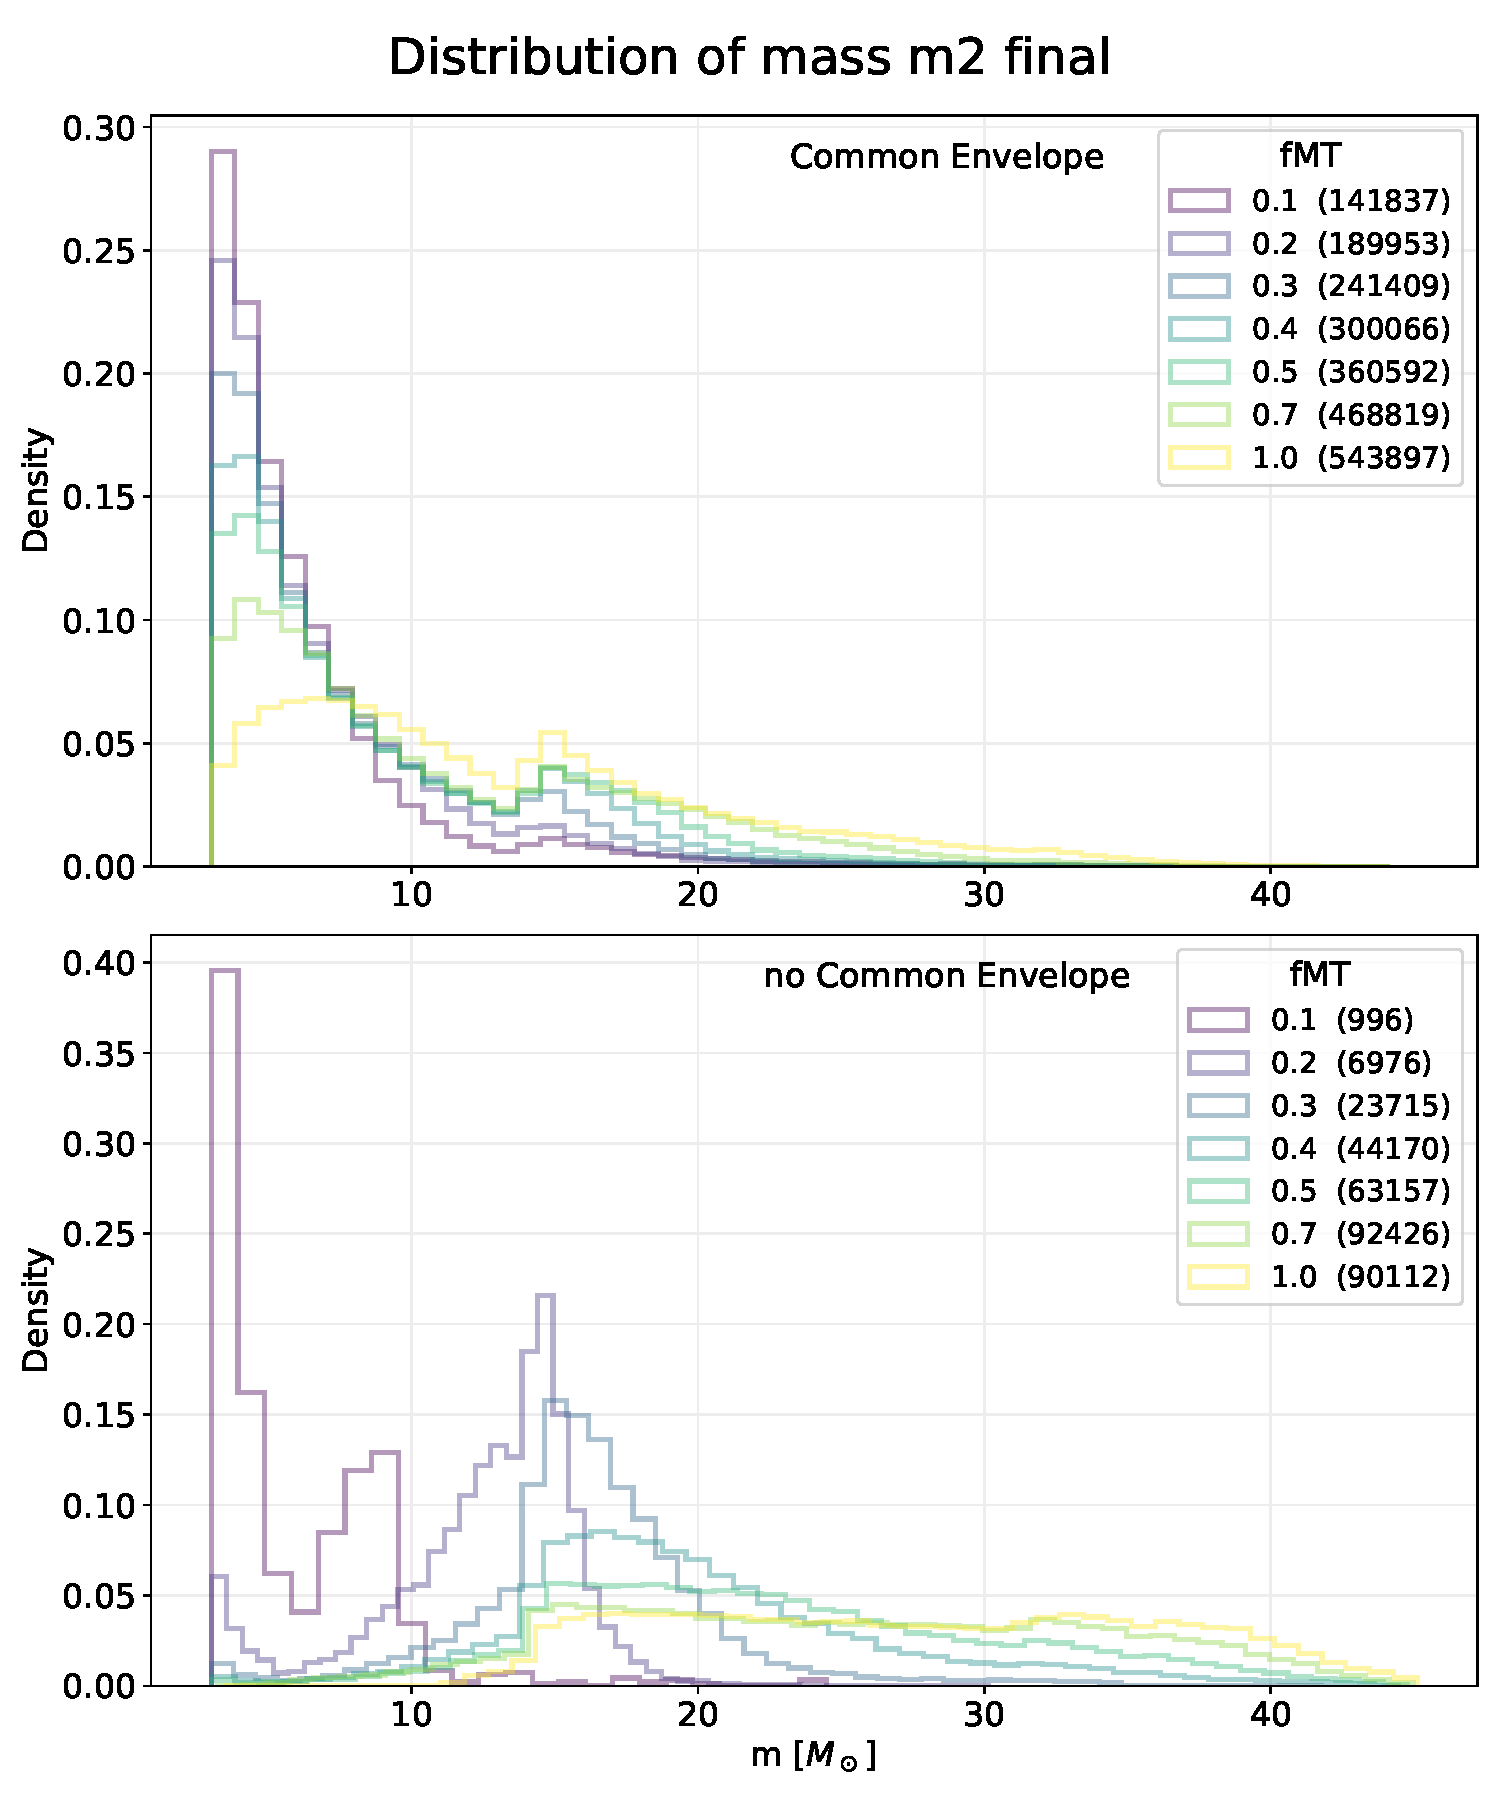
\includegraphics[width=0.49\textwidth]{images/assignment2_1/hist_m2_fin_fMT.pdf}
   \vskip 0.3cm
    \caption{Distribution of initial and final mass for \(m_1\) and \(m_2\) as a function of fMT. In the legend, the color related to each  fMT is reported  with the associated number of counts of the histograms. Note that all the metallicities lower or equal than 0.002 are merged. In particular, for each set of distribution, on the top plots are illustrated the normalized histograms for system which enter in Common Envelope, while on the bottom for systems which do not enter.}
    \label{fig:ass2_masses}
\end{figure*}


\begin{figure}[hbp]
    \begin{minipage}[c]{1.0\columnwidth}
    \centering
    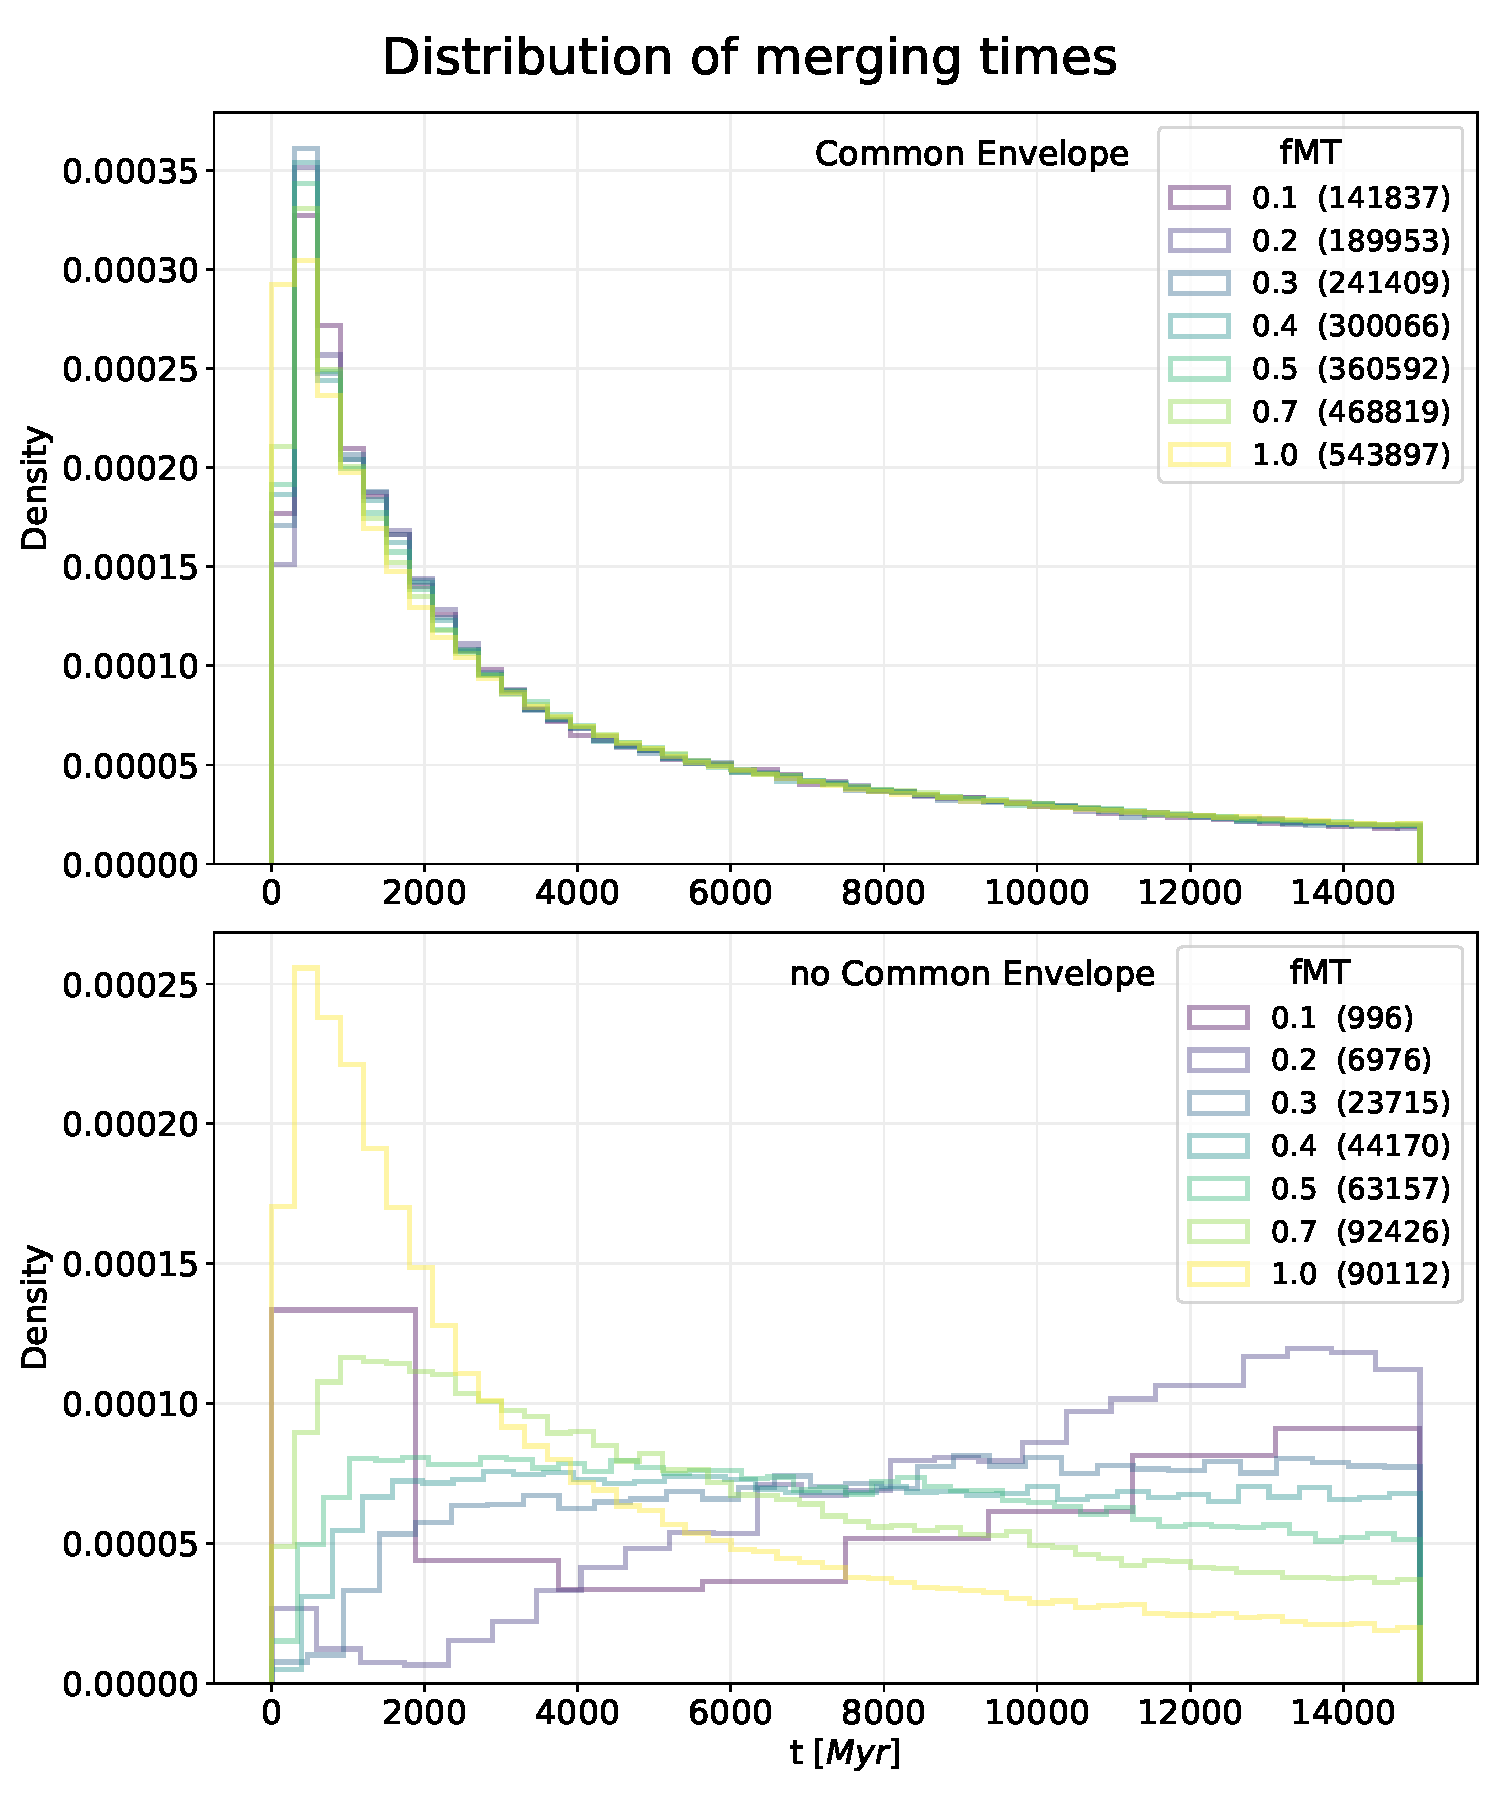
\includegraphics[width=0.9\textwidth]{images/assignment2_1/hist_dtimes_fMT.pdf}
    \caption{Distribution of merging times for different fMT. On the top, the plot for systems which enter in Common Envelope is illustrated, while on the bottom for system which do not.
    In the legend, the color related to each  fMT is reported  with the associated number of counts of the histograms. }
    \label{fig:ass2_1_tmerg}
    \end{minipage}
\end{figure}

%%%%%%%%%%%%%%%%%%%%%%%%%%%%%%%%%%%%%%%%%%%%%%

In Fig. \ref{fig:ass2_frac_CE} we observe that the fraction of systems which enter in Common Envelope decreases for higher values of fMT. In fact, it is essential to have an efficient mass transfer for the system to merge without Common Envelope. Unexpectedly, the fraction is not minimum in fMT\(=1\). Instead, we note no significant trend of the fraction of Common Envelope systems varying the metallicity.

We now consider initial and final mass distribution for CE and nCE systems. 
Star with lower metallicities are expected to be more massive but we do not observe this trend in our analysis. This is due to the fact that initial stellar masses are not uniformly distributed in the simulation code. Indeed, it has been observed that stars in the universe are distributed as a power law. Lighter progenitors predominates with respect to heavier ones independently on metallicity and fMT.

In Fig. \ref{fig:ass2_masses}, we observe that the peak of the distribution of initial masses of the stars in CE systems is around \SI{30}{M_\odot} for the primary and \SI{20}{M_\odot} for the secondary. No trend is observed as a function of fMT. In nCE systems, instead, we observe in both primary and secondary initial masses distributions a shift (\(\sim \: \SI{10/20}{M_\odot}\)) toward higher masses for the peak of the distribution; the shift is more relevant increasing fMT. This is due to the fact that to coalesce in shorter time nCE systems need to be more massive in order to have a faster star evolution. Moreover, the right-hand tail of the distributions becomes longer toward more and more massive stars as a function of fMT.
Considering final masses distribution for CE and nCE, we note that the peak of nCE distributions overlap with the secondary peak of the CE distribution. As far as fMT trend is concerned, analogous consideration can be shared for initial and final masses distributions. 

In Fig. \ref{fig:ass2_1_tmerg} we plot the distributions of delay times as a function of fMT. We observe that for CE systems there is no significant trend to highlight, instead, for nCE systems, increasing fMT cause a significant reduction of merging times. This confirms what we observe in Fig. \ref{fig:ass2_frac_CE}: a high value of fMT is essential to merge without CE. 

In Fig. \ref{fig:ass2_1_q} we plot the distribution of mass ratio \(q\) for initial and final masses of CE and nCE systems. 
Initial mass ratios are more peaked around one for CE systems, while nCE distributions are peaked around 0.6 and presents more extreme mass ratio values, in particular for high fMT. This highlight the fact that systems with similar masses are more likely to enter Common Envelope, while systems with mass ratio further from one are not.
Indeed, a second mass transfer from the secondary to the primary, which is already a compact object, determines the status of the system as CE or nCE. When the mass transfer between the donor and the accretor is unstable, i.e. the donor is heavy with respect to the accretor, the Common Envelope emerges otherwise it does not. Therefore, when we have small value of \(q\), so the secondary is small, nCE systems are more likely to be observed.
For final masses, we observe that nCE tends to shift the mass ratio peak toward one. As a function of fMT we observe, for CE systems, more and more extreme mass ratios toward the right side of the distribution for final masses. While, for nCE systems, we observe less extreme values for mass ratios smaller than one. 
Observing the distribution of ordered mass ratio, we note that for CE system final masses are less peaked at one with respect to initial masses. For nCE system, we observe that final masses gets strongly peak at one with respect to initial masses, especially for high fMT. 

In Fig. \ref{fig:ass2_1_scatterplot} we plot the scatter plot of \(m_1\) vs \(m_2\) in order to understand the origin of extreme mass ratios observed in Fig. \ref{fig:ass2_1_q}. We can see that, for CE systems, extreme mass ratios above one in final masses are caused by small primary masses.  Furthermore, for nCE systems, we can see that extreme mass ratios below one in final masses are caused by small secondary masses. Moreover, we observe an empty region above the bisector in the scatter plot of final masses for Common Envelope systems. 

Eventually, the distribution of semi-major axis for different fMT and metallicities are shown in Fig. \ref{fig:ass2_1_sep}. We observe no significant trend varying either the mass transfer efficiency or the metallicity. However, as expected Common Envelope is proved to shrink the semi-major axis as can be seen by looking at the right and left tail of the distributions. 



\begin{figure*}[htp]
    \centering
    %\begin{minipage}[c]{2.0\columnwidth}
    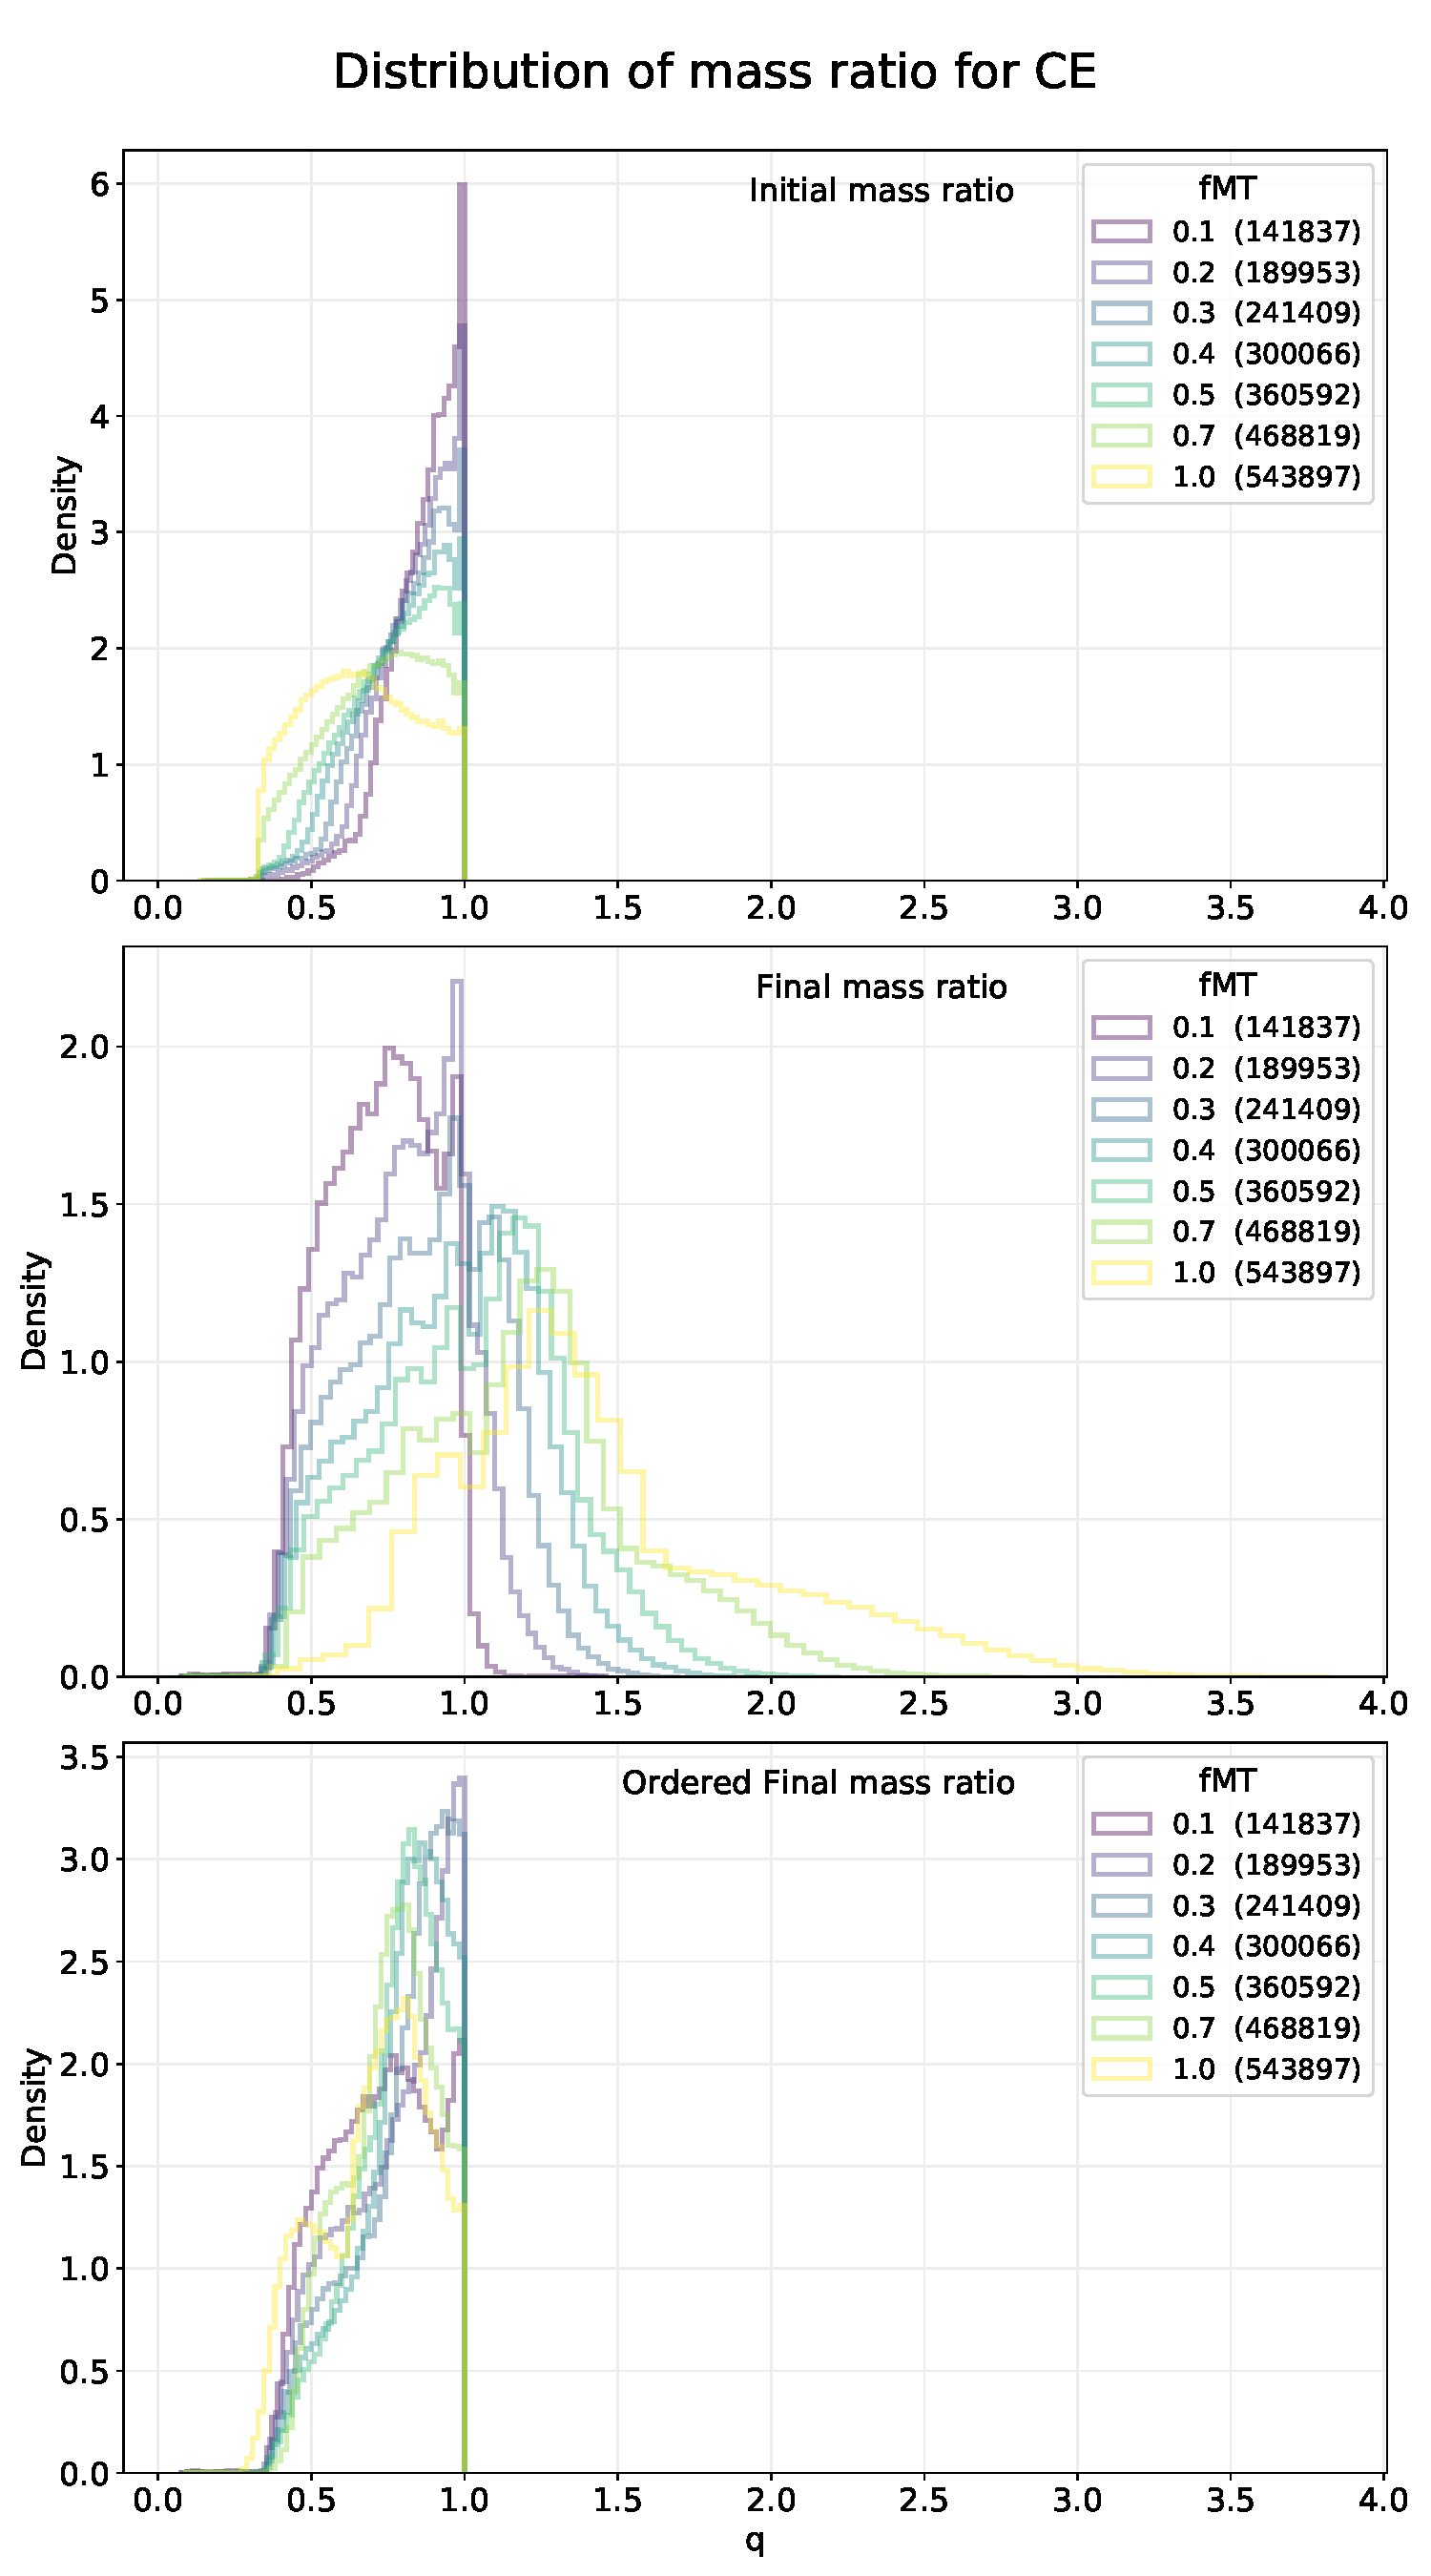
\includegraphics[width=0.49\textwidth]{images/assignment2_1/hist_q_fMT_CE.pdf}
    \hskip 1mm
   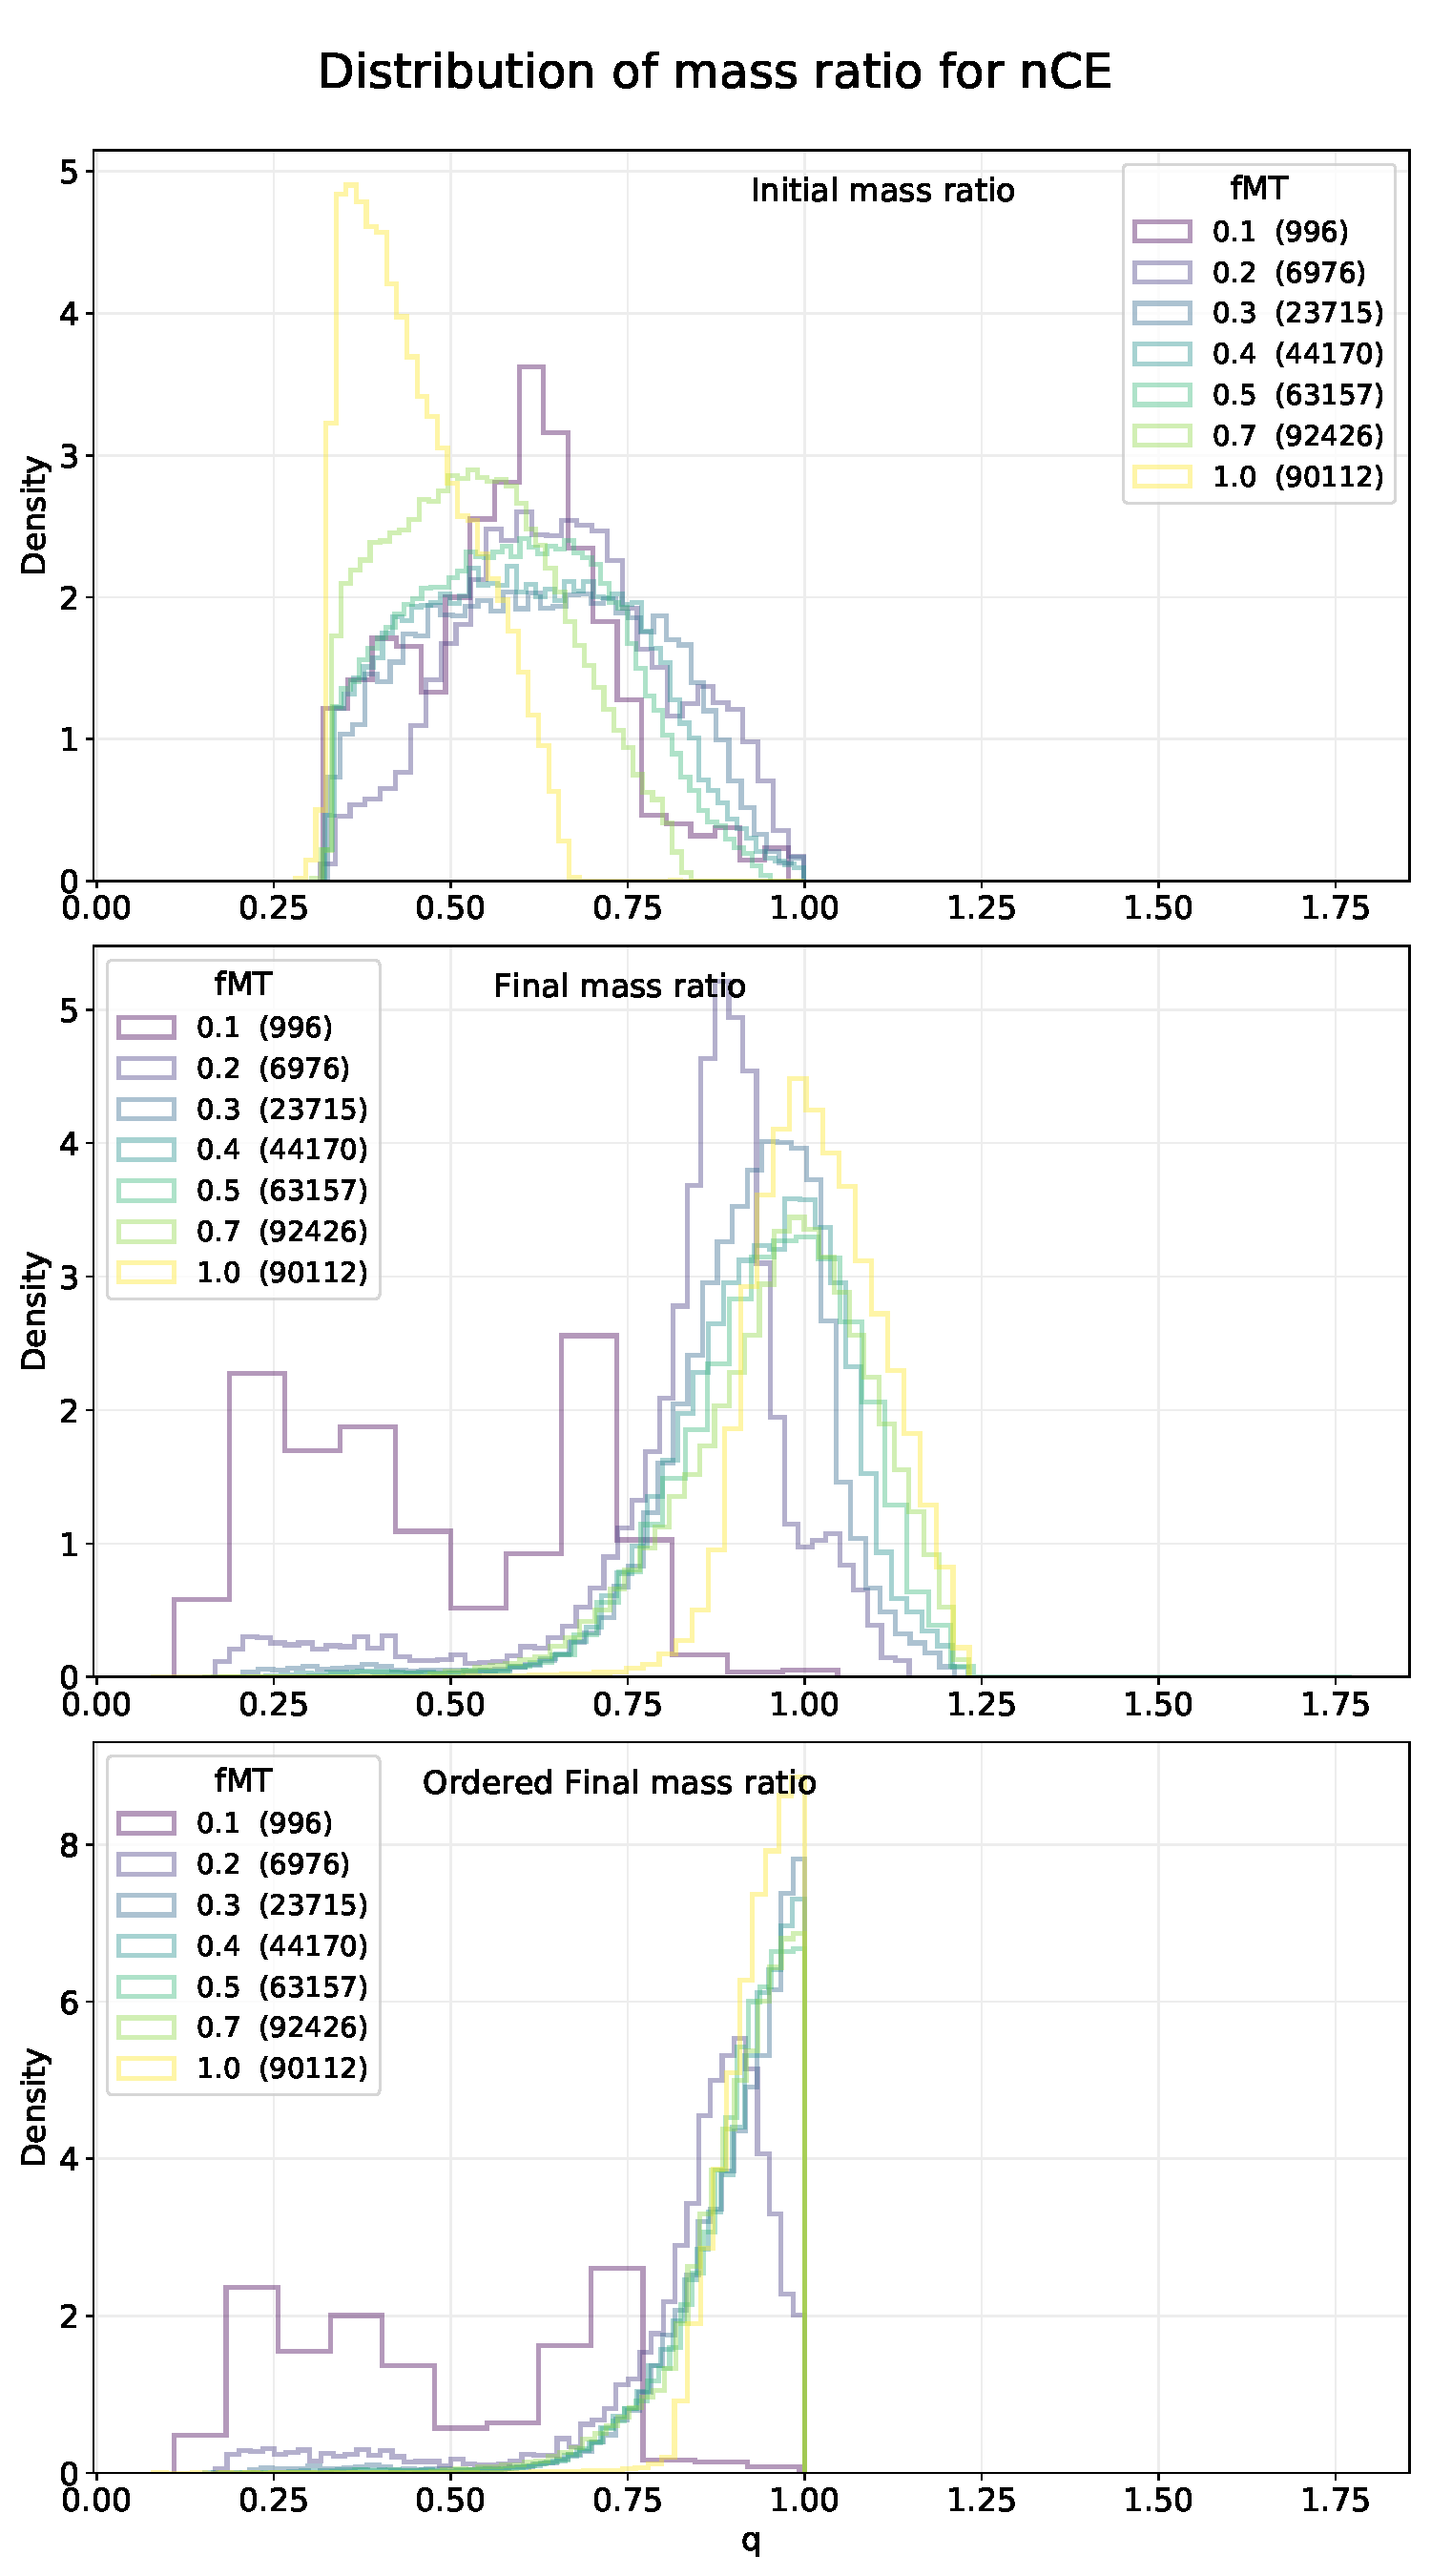
\includegraphics[width=0.49\textwidth]{images/assignment2_1/hist_q_fMT_nCE.pdf}
    \caption{Distribution of mass ratio \(q=m_2/m_1\) for different fMT with all the metallicities lower or equal than 0.002 are merged. 
    On the left, we illustrate the distribution of mass ratio for systems which enter in Common Envelope, while on the right for systems which do not. 
    In particular, for each kind of system, on the top, the plot for initial mass ratio is illustrated. On the middle, we illustrate the plot for final mass ratio, while on the bottom we illustrate the final mass ratio plot where the masses \(m_1\) and \(m_2\) are ordered such that is always satisfied the condition \(m_1>m_2\). In the legend, the color related to each fMT is reported  with the associated number of counts of the histograms.}
    \label{fig:ass2_1_q}
    %\end{minipage}
\end{figure*}

\vspace{1cm}

\section{Conclusions}
In this project, we analyze a set of about \(10^9\) massive binary system generated  with  the  population  synthesis  code  MOBSE. Data has been analyzed on a remote machine with a Python script optimized for handling efficiently the massive amount of simulated data. Several histograms and plots has been produced in order to investigate relevant trends and correlations in Binary Black Holes formation as far as metallicity, mass transfer efficiency and Common Envelope are concerned.  In this report we show only the most relevant plots, while the complete set of plots and the scripts can be found in the following GitHub repository \cite{git}. 
Results shown substantially confirms our theoretical expectations proving our analysis to be free from significant criticalities. 
As discussed in Sec. \ref{sec:results}, some interesting features emerge from plotted distributions of masses, mass ratios and merging times, such as for example unexpected trends observed in Fig. \ref{fig:ass2_frac_CE} and Fig. \ref{fig:ass2_1_scatterplot}. 
Further and deeper analysis are needed to confirm and understand these features.












\begin{figure*}[htp]
    \centering
    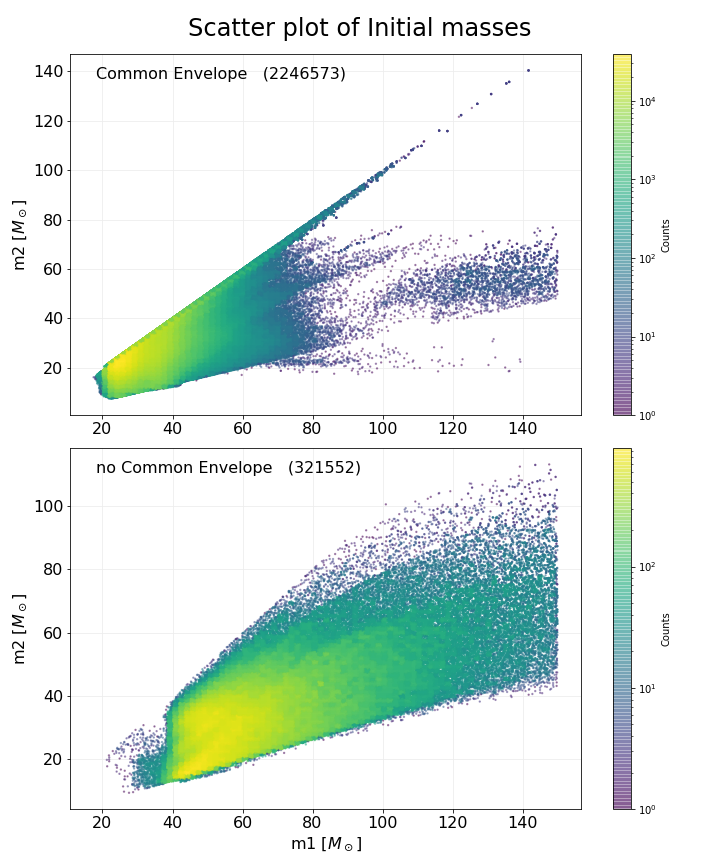
\includegraphics[width=0.44\textwidth]{images/assignment2_1/scatterInitial_masses.png} 
    \hskip 1mm
   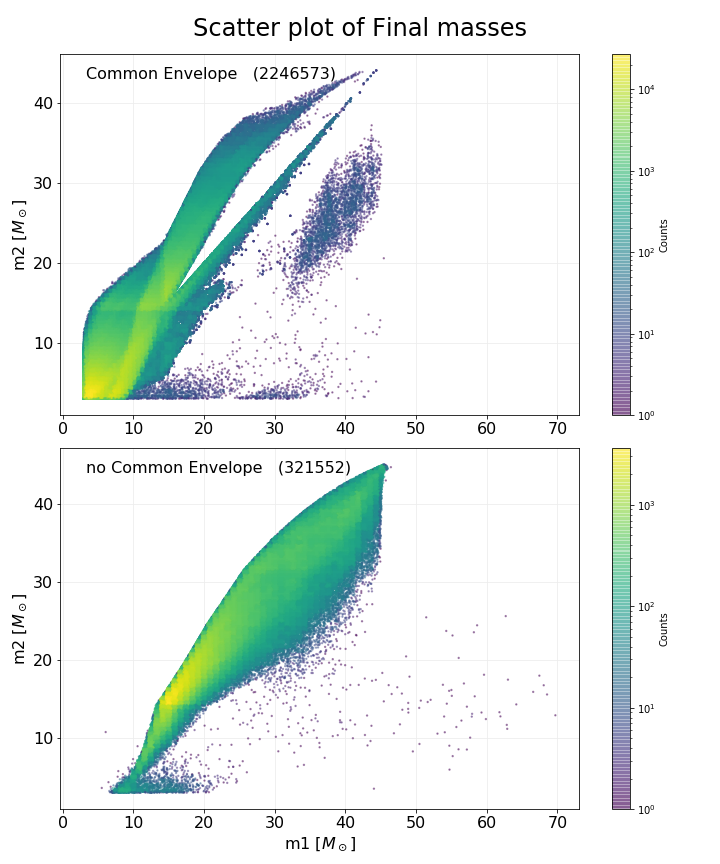
\includegraphics[width=0.44\textwidth]{images/assignment2_1/scatterFinal_masses.png}
   \vskip -0.2cm
 \caption{Scatter plot of initial and final masses for all fMT and all metallicities lower or equal than 0.002.
    On the left, we illustrate the scatter plots for initial and final masses for systems which enter in Common Envelope, while on the right for systems which do not enter in Common Envelope. 
    In the plot, the number of points in the scatter plot is reported. }
    \label{fig:ass2_1_scatterplot}
\end{figure*}
\begin{figure*}[hp]
    \centering
    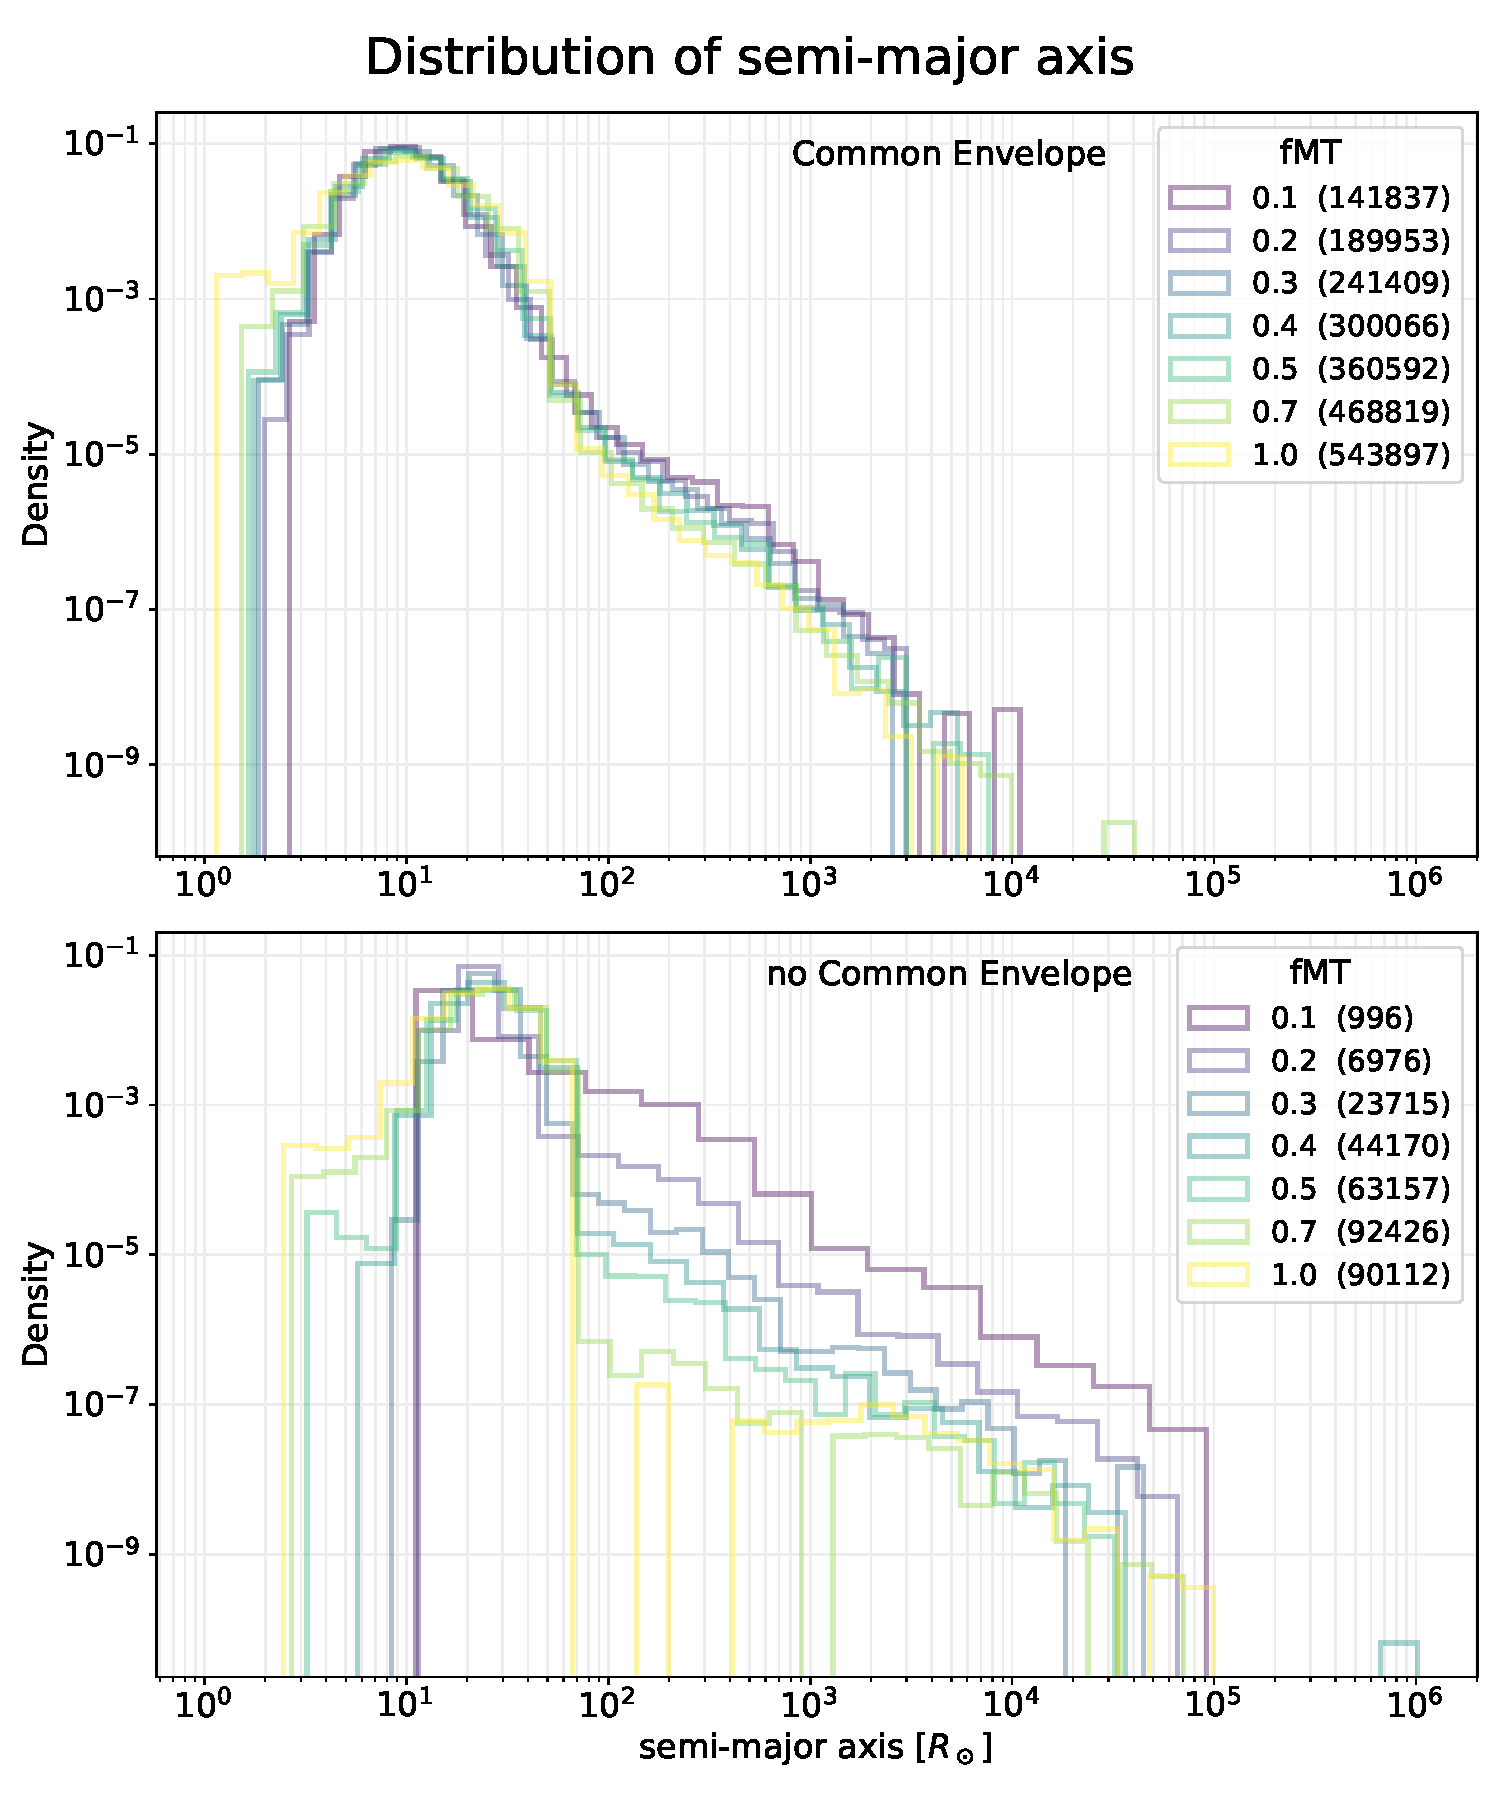
\includegraphics[width=0.49\textwidth]{images/assignment2_1/hist_sep_fMT.pdf}
    \hskip 1mm
   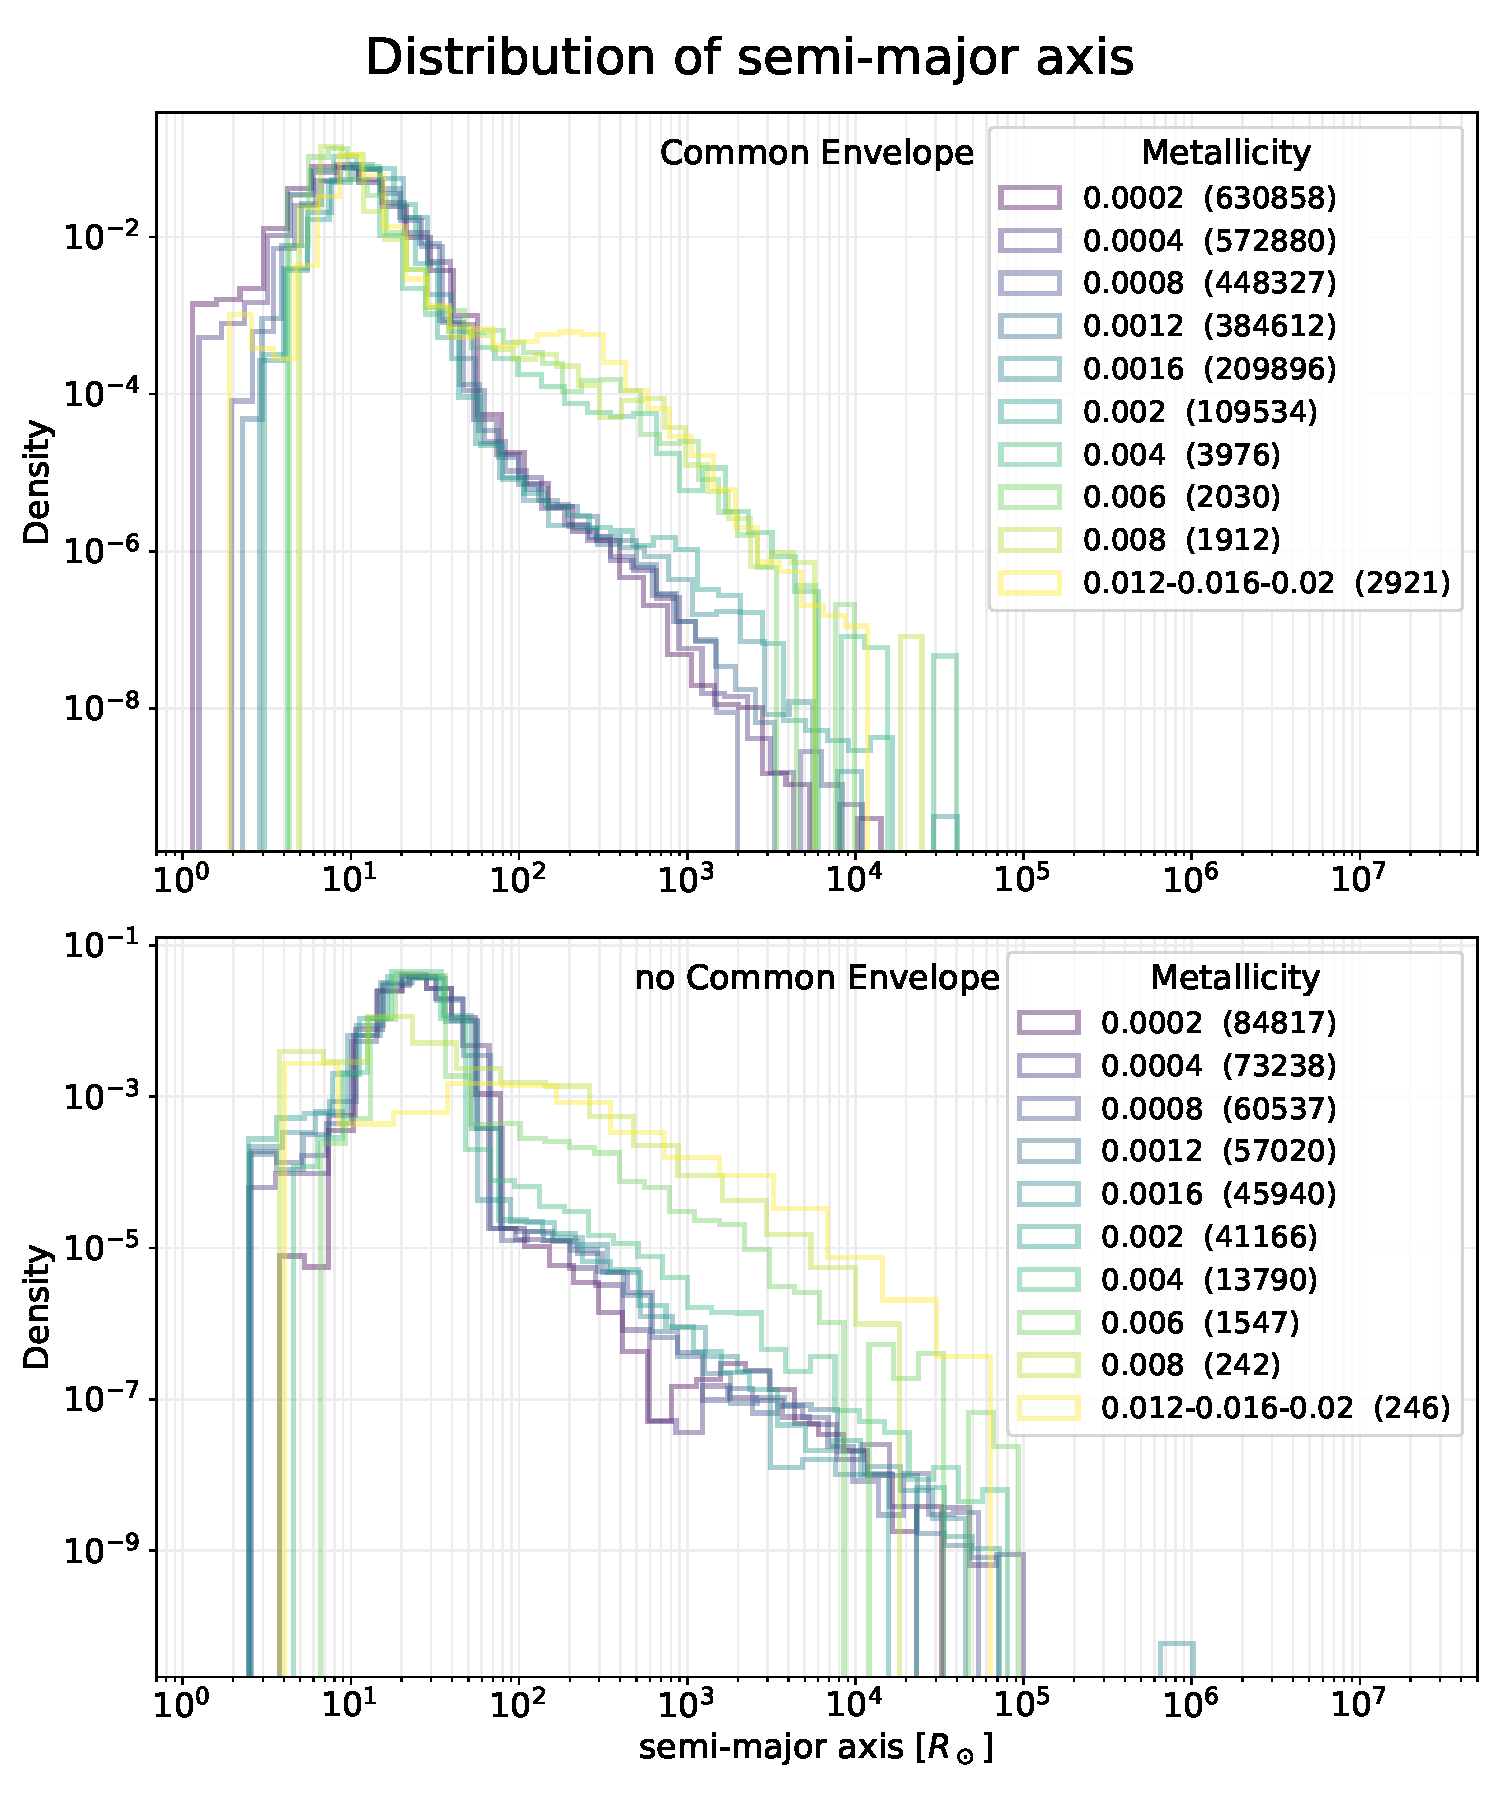
\includegraphics[width=0.49\textwidth]{images/assignment2_1/hist_sep_metal.pdf}
   \vskip -0.2cm
    \caption{ Distribution of semi-major axis. On the left, we illustrate the distributions for different fMT (with all the Z lower or equal than 0.002 merged), while on the right for different metallicities (with all the data for different fMT merged). For each of them, on the top the plot for systems go through Common Envelope is illustrated, while on the bottom for system which do not go. In the legend, the color related to each  fMT, or Z, is reported  with the associated number of counts of the histograms. }
     \label{fig:ass2_1_sep}
\end{figure*}

\clearpage


\nocite{mapelli2018astrophysics}
\nocite{dina}
\nocite{2018MNRAS.480.2011G}
\nocite{2020ApJ...891..141G}
\nocite{2018MNRAS.474.2959G}
\nocite{2012ApJ...759...52D}
\nocite{2019MNRAS.490.3740N}

\printbibliography
\vspace{0.65cm}

\end{document}


